\documentclass[11pt,3p,review,authoryear]{elsarticle}

% use packages
% \usepackage{ecrc} %required for elsarticle https://www.elsevier.com/researcher/author/policies-and-guidelines/latex-instructions
\usepackage[utf8]{inputenc}
\usepackage{amsmath}
\usepackage{amsthm}
\usepackage{amsfonts}
\usepackage{amscd}
\usepackage{amssymb}
\usepackage{natbib}
\usepackage{url}
\usepackage[table,xcdraw,usenames]{xcolor}
%\usepackage[usenames]{color}

\usepackage{graphicx}
\usepackage{subcaption}
\usepackage{mathtools}
\usepackage{enumitem}
\usepackage{bm}
\usepackage{comment}
\usepackage{pdfpages}

\usepackage{hyperref}
\usepackage{caption}
\usepackage{float}
%\usepackage[caption = false]{subfig}
\usepackage{tikz}
\usepackage{multirow}
\usepackage[linesnumbered, ruled,vlined]{algorithm2e}
\usepackage{pdflscape}
\usepackage{etoolbox}

%\AtBeginEnvironment{align}{\setcounter{equation}{0}} % https://tex.stackexchange.com/questions/349247/how-do-i-reset-the-counter-in-align

% margin setup
\usepackage{geometry}
\geometry{margin=0.8in}

% function definition
\newcommand{\V}{\textbf{V}}
\newcommand{\weight}{\pi}
\newcommand{\ret}{\textbf{r}}
\newcommand{\y}{\textbf{y}}
\newcommand{\w}{\textbf{w}}
\newcommand{\x}{\textbf{x}}
\newcommand{\dbf}{\textbf{d}}
\newcommand{\X}{\textbf{X}}
\newcommand{\Y}{\textbf{Y}}
%\newcommand{\L}{\textbf{L}}
\newcommand{\Hist}{\mathcal{H}}
\newcommand{\Prob}{\mathbb{P}}
\def\mbf#1{\mathbf{#1}} % bold but not italic
\def\ind#1{\mathrm{1}(#1)} % indicator function
\newcommand{\simiid}{\stackrel{iid}{\sim}} %[] IID 
\def\where{\text{ where }} % where
\newcommand{\indep}{\perp \!\!\! \perp } % independent symbols
\def\cov#1#2{\mathrm{Cov}(#1, #2)} % covariance 
\def\mrm#1{\mathrm{#1}} % remove math
\newcommand{\reals}{\mathbb{R}} % Real number symbol
\def\t#1{\tilde{#1}} % tilde
\def\normal#1#2{\mathcal{N}(#1,#2)} % normal
\def\mbi#1{\boldsymbol{#1}} % Bold and italic (math bold italic)
\def\v#1{\mbi{#1}} % Vector notation
\def\mc#1{\mathcal{#1}} % mathical
\DeclareMathOperator*{\argmax}{arg\,max} % arg max
\DeclareMathOperator*{\argmin}{arg\,min} % arg min
\def\E{\mathbb{E}} % Expectation symbol
\def\mc#1{\mathcal{#1}}
\def\var#1{\mathrm{Var}(#1)} % Variance symbol
\def\checkmark{\tikz\fill[scale=0.4](0,.35) -- (.25,0) -- (1,.7) -- (.25,.15) -- cycle;} % checkmark
\newcommand\red[1]{{\color{red}#1}}
\def\bs#1{\boldsymbol{#1}}
\def\P{\mathbb{P}}
\def\var{\mathbf{Var}}
\def\naturals{\mathbb{N}}
\def\cp{\overset{p}{\to}}
\def\clt{\overset{\mathcal{L}^2}{\to}}

\setcounter{tocdepth}{4}
\setcounter{secnumdepth}{4}

\newtheorem{corollary}{Corollary}
\newcommand{\ceil}[1]{\lceil #1 \rceil}
\newcommand{\norm}[1]{\left\lVert#1\right\rVert} % A norm with 1 argument
\DeclareMathOperator{\Var}{Var} % Variance symbol

\newtheorem{cor}{Corollary}
\newtheorem{lem}{Lemma}
\newtheorem{thm}{Theorem}
\newtheorem{defn}{Definition}
\newtheorem{prop}{Proposition}
\theoremstyle{definition}
\newtheorem{remark}{Remark}
\hypersetup{
  linkcolor  = blue,
  citecolor  = blue,
  urlcolor   = blue,
  colorlinks = true,
} % color setup

% proof to proposition 
\newenvironment{proof-of-proposition}[1][{}]{\noindent{\bf
    Proof of Proposition {#1}}
  \hspace*{.5em}}{\qed\bigskip\\}
% general proof of corollary
  \newenvironment{proof-of-corollary}[1][{}]{\noindent{\bf
    Proof of Corollary {#1}}
  \hspace*{.5em}}{\qed\bigskip\\}
% general proof of lemma
\newenvironment{proof-of-lemma}[1][{}]{\noindent{\bf
Proof of Lemma {#1}}
\hspace*{.5em}}{\qed\bigskip\\}

\allowdisplaybreaks

\journal{International Journal of Forecasting}

\bibliographystyle{plainnat}
%\bibliographystyle{model5-names}
\biboptions{longnamesfirst}
 
\begin{document}

\begin{frontmatter}

\title{Volatility Forecasting Using Similarity-based Parameter Correction and Aggregated Shock Information}

\begin{abstract}
  We develop a procedure for forecasting the volatility of a time series immediately following a news shock.  Adapting the similarity-based framework of \citet{lin2021minimizing}, we exploit series that have experienced similar shocks.  We aggregate their shock-induced excess volatilities by positing the shocks to be affine functions of exogenous covariates.  The volatility shocks are modeled as random effects and estimated as fixed effects.  The aggregation of these estimates is done in service of adjusting the $h$-step-ahead GARCH forecast of the time series under study by an additive term.  The adjusted and unadjusted forecasts are evaluated using the unobservable but easily-estimated realized volatility (RV).  A real-world application is provided, as are simulation results suggesting the conditions and hyperparameters under which our method thrives.
\end{abstract}

\begin{keyword}
  GARCH \sep 
 Prospective forecasting \sep 
 Volatility \sep 
ARMA \sep 
Risk
\end{keyword}

\end{frontmatter}

\section{Introduction}

Reacting to a seemingly unprecedented event might involve the question: what, if anything, does it resemble from the past?  Such might be the case with event-driven investing strategies, where the identification of the event could arise via the news pages or corporate communications and hence contains a qualitative, narrative element \citep{Kenton}.  Matching a current crisis to past events is a problem with unsurprising statistical angles: identification, sample size, weighting, risk, and robustness, among many others.  

In the context of foreign exchange rate market structure, \citet{dominguez2006defines} speculate ``[w]hether news is scheduled or non-scheduled its influence on exchange rates may be related
to the state of the market at the time of the news arrival.  News that arrives during periods of
high uncertainty may have different effects on the exchange rate, than news that arrives in
calmer periods." The authors also note that non-scheduled news may require more time for markets to digest, leading to greater heterogeneity (including but not limited to higher dispersion) of responses.  We take inspiration from these arguments, developing a method suitable to the conditions that typically accompany news shocks. 

In this work we focus on the second central moment of a time series, the volatility.  One of the most important stochastic phenomenon of positively-valued time series $(P_{t})_{t\in\mathbb{N}}$, especially financial time series, is the volatility of the return series $(r_{t})_{t\in\mathbb{N}}$.  A financial asset's price series may exhibit behavior that makes inapplicable and uninterpretable the traditional methods of time series analysis.  In contrast, the return series is scale-free \citep{tsay2005analysis}, easily-interpreted, and often at least weakly stationary.  Even if one could construct credible models for describing and forecasting price series and return series, that would not necessarily tell us much about the variability of such forecasts nor enlighten us about the evolution of the variability of $(P_{t})_{t\in\mathbb{N}}$ and $(r_{t})_{t\in\mathbb{N}}$ over time.  The literature on return series predictability based on news has undergone a considerable shift over the past 50 years (see \citet{boudoukh2019information} and references therein).  Whereas once returns were thought to react to specific news events, now stock price movements are believed to be overwhelmingly noise-based.

No matter how a time series or its transformations are modeled, forecasting in the presence of news shocks requires a methodological framework that sensibly incorporates relevant information that has yet to manifest in market price or derivative quantities like volatility.  In this setting, regime-change models (see \citet{bauwens2006regime} and citations therein) are of little use because under the assumption of a known exogenous shock, there is no need to estimate a regime-change time, nor is there data following the exogenous shock event to fit a model.  Asymmetric GARCH models were an early attempt to account for fact that negative returns typically beget greater volatility than positive returns \citep{hansen2012realized}.  Problematically, such models depend upon the observation of a negative return to provide the most updated volatility forecast, but under the circumstances posited herein, no such return has been observed.

Similar problems and more exist for Realized GARCH models \citep{hansen2012realized}, which incorporates observable measures of volatility, known as  ``realized measures", like implied volatility.  Under the assumptions herein, no post-shock data is available, and even if it were, Realized GARCH does not promise to perform well, since Black-Scholes implied volatility is a biased estimator of volatility \citep{mayhew1995implied, christensen1998relation}, with the bias increasing in times of crises, when options are likely to be out-of-the-money.  GARCH models have been shown slow to adapt to spikes in volatility \citep{andersen2003modeling}.  \citet{engle2002new} explored the use of implied volatility as an exogenous regressor in a GARCH model, that is, using a so-called GARCH-X model \citep{RePEc:pra:mprapa:100301}.  Realized GARCH aims to solve both the asymmetry problem as well as the slow-reaction problem by introducing a ``measurement equation" as a tool for modeling the contribution to the conditional variance made by the market-implied volatility measure.  The key insight is that a realized measure of volatility will often fail to be independent of the log return of the asset.  Therefore, including the external measure must be done in a way that accounts for this dependence.

The approach herein can be viewed as an attempt to sidestep the functional complexity posited by Realized GARCH, with its minimum nine parameters to estimate \citep{sharma2016forecasting}, by substituting modeling assumptions.  The method herein proceeds under the assumption that similar news events occasion volatility shocks arising from a common shock distribution.  The procedure proposed does not require post-shock information like returns or market-implied quantities from the time series under study.  Hence, we also avoid questions about what realized measure to use and when as well as questions about the usefulness of high-frequency data, although these remain intriguing avenues for future work.

% COMMENTING OUT THE FOLLOWING PARAGRAPH BECAUSE IT BELONGS IN DISSERTATION ONLY
\begin{comment}
  When $(P_{t})_{t\in\mathbb{N}}$ is positive, as one would expect of a price series, the percentage change over any interval of length $k\in\mathbb{N}$ can be approximated by $\text{log}(\frac{P_{t+k}}{P_{t}})$, owing to the fact that for any nonnegative real number y, $\text{log}(y+1)\leq y$.  Equality holds at exactly y = 0, corresponding to the case where $P_{t+k} = P_{t}$.  It is easily verified that the approximation works well when the ratio $\frac{P_{t+k}}{P_{t}} \in (.85,1.15)$, a return absolute value of $15\%$ or less.  The daily log return series $\text{log}(\frac{P_{t+1}}{P_{t}})$, however, not only provides an approximation to the daily return; the logarithm of a price series has the helpful property of being supported on $\mathbb{R}$.  Partly due to that, it earns a pedigree for its role in geometric Brownian motion, the foundation of much of modern financial mathematics, including the Black-Sholes differential equation \citep{tsay2005analysis}.  Additionally, the log transformation is a tried-and-true variance-reduction technique for heteroskedastic data \citep{faraway2016extending} and non-stationary time series.  In many applications, the log return of a positive time series will allow us to reject the null of a unit-root process using the methods pioneered in \citet{dickey1979distribution} and \citet{dickey1981likelihood}, thus paving the way for the vast family of autoregressive-moving-average models.
\end{comment}

The primary methodological tool presented in this work is fixed effect estimation followed by an appropriate procedure for pooling those estimates.  The use of fixed effect estimation for the study of structural shocks has a pedigree in macroeconomic analysis (\citet{romer1989does} cited in \citet{kilian2017structural}; see also discussion of determinstic exogenous events in \citet{engle2001good}).  In the forecasting literature, the term ``intercept correction'' has come to refer to a modeling technique in which nonzero errors are explicitly permitted \citep{hendry1994theory, clements1998forecasting}.  They summarize the literature as distinguishing two families of intercept correction: intercept corrections that attempt to account for future events, without hard-coding an ad-hoc adjustment into the model specification, and second, intercept corrections that attempt to adjust for persistent misspecification using past errors.  \citet{guerron2017macroeconomic} use weighted subsets of a scalar series' own past to correct forecast errors by an additive term. \citet{dendramis2020similarity} a introduces a similarity-based forecasting procedure for time-varying coefficients of a linear model. \citet{foroni2022forecasting} employ a form of intercept correction in order to adjust forecasts to the COVID-19 shock in the spring of 2020 based on the proportional misses of the same model applied to the Great Recession.

A researcher interested in forecast adjustment can choose between procedures that automated or non-automated, a variety of choices for the collection of data assembled to perform the correction, whether the data is internal (the time series itself) or external, the parametric term to be corrected (e.g. intercept, coefficients), if any, as well as the correction function (i.e. the mapping from the data to the corrective term), including the weighting applied to the assembled data (e.g. Nearest-Neighbor, arithmetic mean, kernel methods).

Our procedure is an automated procedure for intercept adjustments using either data internal or external to the time series under study.  The correction function, as we shall see, involves an optimization step inspired by the causal inference literature.  In particular, in \citet{abadie2010synthetic}, the authors build upon previous work in causal inference whereby a treatment effect can be estimated by creating a synthetic time series that that represents either the treatment or control unit.  The synthetic unit is constructed using a convex combination of the so-called donor series.  The particular convex combination employed is a function of the distance between the time series under study and the donors.  \citet{lin2021minimizing} adapted these methods for the purpose of prediction.  Their 1-step-ahead forecasts use distance-based-weighting to pool shock estimates from similar series according to the donor series' similarity to the series under study.  Their approach does not take into account the ARCH effects commonly observed in time series, especially financial times series, leaving unaccounted for the variability that accompanies predictions of a heteroskedastic time series.  In this present study, we focus on only volatility forecasting.  We furthermore depart from \citet{lin2021minimizing} framework by weighting series not by their covariates (which would be most appropriate for estimating the parameters of time series' mean model) but by their volatility profile.  

Outside of \citet{lin2021minimizing}, we know of no prior work that both introduces a parametric specification for nonzero errors and introduces a procedure for weighting appropriately the nonzero errors of similar shocks.  Likewise, we are not familiar with any prior work that attempts to account for anticipated nonzero errors using an explicit parametric adjustment.  This current work is a contribution to the forecast adjustment literature but also aims for the virtues of robustness, risk-minimization, and model interpretability, akin to the departures from nearest neighbors discussed in \citet{abadie2021penalized}.  \citet{guerron2017macroeconomic}, citing previous work, discuss that intercept corrections find their theoretical basis in the occurrence of structural breaks, whereas Nearest-Neighbor methods, being nonparametric, are theoretically more adept at accounting for nonlinearity.  By using convex combinations of donor pool quantities to adjust forecasts, we are generalizing Nearest-Neighbor methods while also providing robustness, risk-minization, and model interpretability.

In order to motivate our procedure, we show how the aggregation of estimated excess volatilities from donors in the donor pool works when the correction function is the arithmetic mean.  As we see in Figure \ref{fig:arith_mean_example_introduction}, the arithmetic mean of excess volatilities provides perhaps the most straightforward and intuitive way of aggregating information from similar events.  Taking the average also coincides with the $K$-Nearest-Neighbor estimator, where $K$ is equal to the number of donors in the donor pool. Although using the arithmetic mean is intuitive and enjoys some empirical track record, its grounding in theory is much less impressive \citep{timmermann2006forecast}.  Our method assumes a credible, parsimonious parameterization in which the shock is an affine transformation of several key covariates.  The key intuition behind this shock parameterization is that as the strength of the linear signal increases relative to the idiosyncratic error, the GARCH estimation of these effects increases in accuracy.  From this, it follows that the aggregated shock estimate increases in accuracy. 

  \begin{figure}[h]
    \begin{center}
      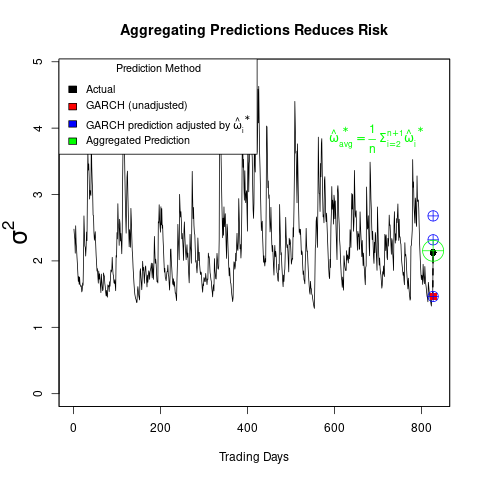
\includegraphics[scale=.7]{simulation_plots/USE_in_paper_simulation_plot_arithmetic_mean.png}
      \caption{The time series experiences a volatility shock at a uniformly distributed point in the interval [756, 2520] trading days, corresponding to trading years on the interval [3,10].  We have truncated the series after $T^{*}+1$.  The GARCH prediction fails even to approach the volatility spike at $T^{*}+1$, as do some adjusted predictions.  In contrast, the GARCH forecast adjusted by $\overline{\hat\omega^{*}}$, the arithmetic mean of the estimated shocks, recovers the shock in the time series under study.} 
      \label{fig:arith_mean_example_introduction}
      \end{center}
    \end{figure}

\section{Setting}
\label{section2}

\subsection{A Primer on GARCH}
We define the log return of an asset between $t-1$ and $t$ as $r_{t} = \text{log}(\frac{P_{t+1}}{P_{t}})$, where $P_{t}$ denotes the price at time $t$.  The class of ARIMA($p,d,q$) models  \citep{box2013box} provides a framework for postulating and quantifying the autoregressive structure of $r_{t}$, all within the framework of frequentist statistics.  These models assume a certain dependence structure between $r_{t}$ and $(r_{k})_{k\leq t}$, yet their errors --- often called innovations in the financial time series context due to how they represent the impact of new information --- are nevertheless assumed to be i.i.d. with mean zero and constant variance.  The ARCH \citep{engle1982autoregressive} and GARCH \citep{bollerslev1986generalized} models provide elegant alternatives to the homoskedasticity assumption.  In fact, the GARCH framework in its most basic form disregards $r_{t}$ and instead turns its interest to the series $r_{t}^{2}$ (when properly centered, i.e. after assuming a mean-model for returns).  

To that end, let $a_{t} = r_{t} - \mu_{t}$, where $\mu_{t}$ is the mean of the log return series $r_{t}$.  We thus derive a mean-zero process $(a_{t})_{t\in\mathbb{N}}$ with the property that $\E[a^{2}_{t}] = \mrm{Var}[a_{t}]$.  Under the assumption of time-invariant volatility, the series $a_{t}^{2}$ should exhibit no autocorrelation at any lag $\ell\geq1$.  This assumption motivates tests for so-called ARCH effects, that is, tests for the clustering of volatility.  These tests explore the alternative hypothesis that $\sigma_{t}^{2}$ is not only a time-varying parameter but furthermore a function of past squared residuals of the mean model.  In particular, the ARCH($m$) model is an autoregressive model in which $\sigma_{t}^{2}$ is fitted using a linear combination of the past $m$ values of $r_{t}^{2}$.  The GARCH($m,s$) framework take this one step further but modeling $\sigma_{t}^{2}$ as a linear combination of the past $m$ values of $r_{t}^{2}$ and well as the past $s$ values of $\sigma_{t}^{2}$.  In functional form, a GARCH process (sometimes called a strong GARCH process \citep[p. 19]{francq2019garch}) is given by

\begin{align*}
&\sigma_{t}^{2} = \omega + \sum^{m}_{k=1}\alpha_{k}a^{2}_{t-k} + \sum_{j=1}^{s}\beta_{j}\sigma_{t-j}^{2}\\
&a_{t} = \sigma_{t}\epsilon_{t}\\
&\epsilon_{t} \simiid E[\epsilon_{t}]=0, Var[\epsilon_{t}] = 1\\
&\forall k,j, \alpha_{k},\beta_{j}\geq 0\\ 
&\forall t, \omega, \sigma_{t} > 0 \text { .} 
\end{align*}
Assuming further that $\sigma^{2}_{t}$ depends on a vector of exogenous covariates $\x_{t}$, we have a  GARCH-X$(m,s)$.  The volatility equation then becomes 

\begin{align}
&\sigma_{t}^{2} = \omega+ \sum^{m}_{k=1}\alpha_{k}a^{2}_{t-k} + \sum_{j=1}^{s}\beta_{j}\sigma_{t-j}^{2} + \gamma^{T}\x_{t} \text{ .}\label{GARCH-X}
\end{align}

% https://latex-tutorial.com/matrices-in-latex/
% https://www.math-linux.com/latex-26/faq/latex-faq/article/how-to-write-matrices-in-latex-matrix-pmatrix-bmatrix-vmatrix-vmatrix

\subsection{Model setup}
\label{modelsetup}
We will suppose that a researcher has multivariate time series data $\y_{i,t} = (r_{i,t}$, $\x_{i,t}$), $t = 1,$ $\ldots,  T_i$ and $i = 1, \ldots, n+1$, where $r_{i,t}$ is a scalar response (typically the log return of a financial asset) and  $\textbf{v}_{i,t}$ is a vector of covariates such that $\x_{i,t}|\mathcal{F}_{i,t-1}$ is deterministic.  Suppose that the analyst is interested in forecasting the volatility of $r_{1,t}$, the first time series in the collection.  We require that each time series $\y_{i,t}$ is subject to a news event following $T^*_i \leq T_{i} + 1$ and before witnessing $T^*_i+1$.  We are implicitly leveraging the fact that financial assets are heavily traded during market hours, yet only thinly traded (if traded at all) outside market hours.  In contrast, the arrival of market-moving news does not obey any such restrictions.  In light of the foregoing, we can denote our collection of GARCH volatility equations of interest using the following notation

\begin{align*}
&\sigma_{i,t}^{2} = \omega_{i} + \sum^{m_{i}}_{k=1}\alpha_{i,k}a^{2}_{i,t-k} + \sum_{j=1}^{s_{i}}\beta_{i,j}\sigma_{i,t-j}^{2} + \gamma_{i}^{T} \x_{i,t} \text{ }. \\
\end{align*}
Let $I(\cdot)$ be an indicator function.  Let $T_i$ denote the time length of the time series $i$ for $i = 1, \ldots, n+1$, and let $T_i^*$ denote the largest time index prior to the arrival of the news shock, with $T_i^* < T_i$.  Let $\delta, \x_{i,t} \in \mathbb{R}^{p}$.  For $t= 1, \ldots, T_i$ and $i = 1, \ldots, n+1$, the model $\mc{M}_1$ is defined as 
\begin{align*}
  \mc{M}_1 \colon \begin{array}{l}
     \sigma^{2}_{i,t} = \omega_{i} + \omega^{*}_i + \sum^{m_{i}}_{k=1}\alpha_{i,k}a^{2}_{i,t-k} + \sum_{j=1}^{s_{i}}\beta_{i,j}\sigma_{i,t-j}^{2} + \gamma_{i}^{T} \x_{i,t} \text{ }\\[.2cm]
     a_{i,t} = \sigma_{i,t}((1-D^{return}_{i,t})\epsilon_{i,t} + D^{return}_{i,t}\epsilon^{*}_{i})\\[.2cm]
    \omega_{i,t}^{*} = D^{vol}_{i,t}[\mu_{\omega^{*}}+\delta'\mbf{x}_{i, t}+ u_{i,t}],
  \end{array}
  \end{align*}
with error structure

  \begin{align*}
    \epsilon_{i,t} &\simiid \mc{F}_{\epsilon} \text{ with }  \; \mrm{E}_{\mc{F}_{\epsilon}}(\epsilon) = 0, \mrm{Var}_{\mc{F}_{\epsilon}}(\epsilon)  = 1  \\
    \epsilon^{*}_{i,t} &\simiid \mc{F}_{\epsilon^{*}} \text{ with }  \; \mrm{E}_{\mc{F}_{\epsilon^{*}}}(\epsilon) = \mu_{\epsilon^{*}}, \mrm{Var}_{\mc{F}_{\epsilon^{*}}}(\epsilon^{*})  = \sigma^2_{\epsilon^{*}}  \\
    u_{i,t} & \simiid  \mc{F}_{u} \text{ with }  \; \mrm{E}_{\mc{F}_{u}}(u) = 0, \mrm{Var}_{\mc{F}_{u}}(u) = \sigma^2_{u}\\
    \epsilon_{i,t} & \indep  \epsilon^{*}_{i,t}  \indep u_{i,t}
    \end{align*}
where $D^{return}_{i,t} = I(t \in \{T_i^* + 1,...,T_i^* + L_{i, return}\})$ and $D^{vol}_{i,t} = I(t \in \{T_i^* + 1,...,T_i^* + L_{i, vol}\})$ and $L_{i,return},L_{i,vol}$ denote the lengths of the log return and volatility shocks, respectively.  Let $\mc{M}_{0}$ denote the subclass of $\mc{M}_{1}$ models such that $\delta \equiv 0$.  Note that $\mc{M}_{0}$ assumes that $\omega^{*}_i$ have no dependence on the covariates and are i.i.d. with $\E[ \omega^{*}_i]=\mu_{\omega^{*}}$.  

Consider the connection between the model above and the factor model from \citet{abadie2010synthetic}, where an untreated unit is governed by:

\begin{align}
Y^{N}_{i,t} = \delta_{t} + \boldsymbol\theta_{t}\textbf{Z}_{i}+\boldsymbol\lambda_{t}\boldsymbol\mu_{i}+\varepsilon_{i,t} \text{ ,} \label{abadie_factor_model}
\end{align}
which happens to nest the GARCH model's volatilty equation (putting aside that $\sigma_{t}$ is latent in the GARCH model) as well as as the ARMA representation of a GARCH model, where

\begin{align*}
\delta_{t} & \sim \omega,  \text{a location parameter shared across donors}\\
\boldsymbol\theta_{t} & \sim \boldsymbol\alpha_{k},  \text{a vector of ARCH parameters and other coefficients shared across donors} \\
\textbf{Z}_{i} & \sim \boldsymbol a_{i,t-k}, \text{a vector of observable quantities specific to each donor} \\
\boldsymbol \lambda_{t} & \sim \boldsymbol\beta_{j}, \text{a vector of GARCH parameters shared across donors} \\
\boldsymbol \mu_{i} & \sim \boldsymbol \sigma_{i,t-j}^{2}, \text{a vector of latent quantities specific to each donor}   \\
\end{align*}
and $\varepsilon_{i,t}$ is idiosyncratic noise, uncorrelated across time and donors.

    \subsection{Volatility Profile of a Time Series}
    \label{Volatility Shock Profile of a Time Series}
    
    In this section, we make a novel contribution to prediction via distance-based weighting by constructing a profile of a time series' volatility, the analogue of a covariate matrix in a synthetic control framework.  The volatility profile for a given GARCH-X process is nothing more than a vector of observable covariates that parameterize a shock.  A collection of $n$ such vectors yields a matrix of $n$ columns.  What distinguishes a volatility profile, principally, is that the time-varying parameters that correspond to the volatility profile are non-zero at only the shock times, whereas no such restriction exists in ($\ref{abadie_factor_model}$).  
    
    Suppose that for each of the $n$ donors, we posit $p$ distinct covariates in the functional form of the shock.  The volatility profile could take the form of the $p \times n$ matrix 

    \begin{equation*}
      \textbf{V}_{t} = 
      \begin{pmatrix}
      \hat\alpha_{1,t} & \hat\alpha_{t,2}  & \cdots & \hat\alpha_{t,n}  \\
      \hat\beta_{1,t} & \hat\beta_{t,2}  & \cdots & \hat\beta_{t,n}  \\
      \vdots  & \vdots  & \ddots & \vdots  \\
      RV_{1,t} & RV_{2,t}  & \cdots & RV_{n,t}  \\
      RV_{1,t-1}  & RV_{2,t-1}  & \cdots & RV_{n,t-1}  \\
      \vdots  & \vdots  & \ddots & \vdots  \\
      IV_{1,t} & IV_{2,t} & \cdots & IV_{n,t} \\
      IV_{1,t-1}  & IV_{2,t-1}  & \cdots & IV_{n,t-1} \\
      \vdots  & \vdots  & \ddots & \vdots  \\
      |r_{1,t}| & |r_{2,t}| & \cdots & |r_{n,t}| \\
      |r_{1,t-1}|  & |r_{2,t-1}|  & \cdots & |r_{n,t-1}| \\
      \vdots  & \vdots  & \ddots & \vdots  \\
      Volume_{1,t}  & Volume_{2,t}  & \cdots & Volume_{n,t} \\
      Volume_{1,t-1}  & Volume_{2,t-1}  & \cdots & Volume_{n,t-1}  \\
      \vdots  & \vdots  & \ddots & \vdots  \\
      \Delta RV_{1,t} & \Delta RV_{2,t}  & \cdots & \Delta RV_{n,t}  \\
      \Delta RV_{1,t-1}  & \Delta RV_{2,t-1}  & \cdots & \Delta RV_{n,t-1}  \\
      \vdots  & \vdots  & \ddots & \vdots  \\
      \end{pmatrix},
      \end{equation*}
      where RV and IV denote realized volatility and implied volatility, respectively.  Covariates chosen for inclusion in a given volatility profile may be levels, log differences in levels, percentage changes in levels, or absolute values thereof, among many choices.

      As shown, $\textbf{V}_{t}$ displays `balance' in that $p$ covariates exist for each of the $n$ donors.  In practice, missing values, corrupted values, or unacceptably extreme or noisy estimates may necessitate some sort of matrix completion, a problem that we do not tackle in this work.  We now turn to the next section, where $\textbf{V}_{t}$ is employed in a procedure to arrive at a forecast adjustment. 
    

\section{Methodology for Similarity-based Parameter Correction}

\subsection{Forecasting}

We present two forecasts:

\begin{align*}
  \text{Forecast 1: } & \hat\sigma^{2}_{unadjusted} = \hat\E[\sigma^{2}_{1,T_{1}^{*}+1}|\mathcal{F}_{T^{*}}] = \hat\omega_{i} + \sum^{m_{i}}_{k=1}\hat\alpha_{i,k}a^{2}_{i,t-k} + \sum_{j=1}^{s_{i}}\hat\beta_{i,j}\sigma_{i,t-j}^{2} + \hat\gamma_{i}^{T} \x_{i,t}\\
  \text{Forecast 2: } & \hat\sigma^{2}_{adjusted} = \hat\E[\sigma^{2}_{1,T_{1}^{*}+1}|\mathcal{F}_{T^{*}}] + \hat\omega^{*} = \hat\omega_{i} + \sum^{m_{i}}_{k=1}\hat\alpha_{i,k}a^{2}_{i,t-k} + \sum_{j=1}^{s_{i}}\hat\beta_{i,j}\sigma_{i,t-j}^{2} + \hat\gamma_{i}^{T} \x_{i,t} + \hat\omega^{*} \text{ .}
\end{align*}

A GARCH model is an ARMA on the squares of the observed scalar time series $a^{2}_{t}$ \citep[][p. 18, p. 46]{tsay2005analysis,francq2019garch}, assuming that $a_{t}$ satisfies fourth-order stationarity.  This fact matters for forecasting because the $h$-step-ahead forecasting function for GARCH model is, just like for an ARMA model, the conditional expectation function, $\mathbb{E}[ \sigma^{2}_{i,T^{*}+h} | \mathcal{F}_{T^{*}}]$, or practically speaking, the estimate thereof, $\hat{\mathbb{E}}[ \sigma^{2}_{i,T^{*}+h} |\mathcal{F}_{T^{*}}]$ \citep{zivot2009practical}.  Here we have presented one-step-ahead forecasts for a GARCH-X(1,1), without loss of generality.  For $h=2,3,4,...$, the conditional expectation is computed recursively, as is standard for iterative autoregressive forecasts.

\subsection{Excess Volatility Estimators}
    \label{Excess Volatility Estimators}
   
    The problem of aggregating estimated donor shocks begins with the data constraints.  Taking the estimated shocks as a given, we essentially observe the pair $(\{\hat\omega^{*}_{i}\}^{n+1}_{i=2},\{\textbf{v}_{i}\}^{n+1}_{i=2})$.  We wish to recover weights $\{\weight_{i}\}^{n+1}_{i=2} \in \Delta^{n}$ leading to favorable forecasting properties.  These weights are used to compute $\hat\omega^{*} \coloneq \sum^{n+1}_{i=2}\weight_{i}\hat\omega^{*}_{i}$, our forecast adjustment term.  Since the $\{\weight_{i}\}_{i=2}^{n+1}$ are computed using $\mathcal{F}_{T^{*}_{i}}$, the set $\{\weight_{i}\}_{i=2}^{n+1}$ is deterministic, $\textit{modulo}$ any stochastic ingredient in the numerical methods employed to approximate $\x_{1,T^{*}}$ using a convex combination of donor covariates.  We will say more about the properties of $\omega^{*}_{i}$ in section $\ref{SVF_properties}$. 

    Following \citet{abadie2003economic,abadie2010synthetic}, let $\|\cdot\|_{\textbf{S}}$ denote any semi-norm on $\mathbb{R}^{p}$, and define

    \begin{align*}
    \{\pi\}_{i=2}^{n+1} = \argmin_{\pi}\|\textbf{v}_{1} - \V_{t}\pi \|_{\textbf{S}} \text{ .}
    \end{align*}
In the forecast combination literature, it is discussed whether the weights employed to aggregate forecasts strive toward and meet various optimality criteria \citep{timmermann2006forecast,wang2023forecast}.  In this work, there are at least two senses of optimal weights that one might be interested in.  First, we can think of optimal weights as a set $\{\weight_{i}\}_{i=2}^{n+1}$ such that $\omega_{1} = \sum^{n+1}_{i=2}\weight_{i}\hat\omega_{i}$, i.e., $\omega_{1}$ is recovered perfectly, as it belongs to convex hull of the estimated shocks. However, $\omega_{1}$ is never revealed to the practitioner, and hence there is no way of verifying the extent to which this condition is satifised.

A more promising aim is finding weights such that $\textbf{v}_{1} = \sum^{n+1}_{i=2}\weight_{i}\textbf{v}_{i}$, meaning that the volatility profile of the time series under study lies within the convex hull of the donor volatility profile.  This condition underwrites asymptotic results in \citet{abadie2010synthetic}, and the intuition there extends to this work: if the shock is parameterized by an affine function of covariates, then finding a linear combination that recreates the shock should serve us well.  Because the method proposed uses a point in $\Delta^{n}$, it is important to head-off possible confusion.  What we are proposing is not a forecast combination method.  What we aggregating and weighting (not combining) is subcomponents of forecasts, not forecasts themselves.  Moreover, from a broader perspective, forecast combination is an inapt term for what is being proposed here.  First, the donor time series do not provide forecasts, nor would forecasts been needed for random variables that have already been realized.  Second and more fundamentally, the theoretical underpinnings of forecast combination, while diverse \citep{wang2023forecast}, are distinct from the setting presumed in this work, where the model family is not in doubt but the parameter values and how they prevail must be learned.

A question naturally arises regarding the uniqueness of weights.  Remarks by \cite{lin2021minimizing, abadie2022synthetic} apply here.  We make additional comments as well. $(\mathbb{R}^{n}, \|\cdot\|)$ is a Chebyshev space, and hence for any element x and any convex set $C\subset \mathbb{R}^{n}$, there exists a unique element $y\in C$ that minimizes $\|x-y\|$.  However, the pre-image of $y$ with respect to a particular operator and constraint set might not be unique.

Let $p', n'$ denote the number of linearly independent rows of $\V_{t}$ and linearly independent columns of $\V_{t}$ respectively.  Let col($\cdot$) denote the column space of matrix, and let Conv($\cdot$) denote the convex hull of a set of vectors.  \\

    \begin{center}
      \begin{tabular}{ | m{3em} | m{7cm}| m{7cm} | } 
        \hline
        & $\textbf{v}_{1}\in \text{Conv}(\text{col}(\V_{t}))$ & $\textbf{v}_{1} \notin \text{Conv}(\text{col}(\V_{t}))$\\ 
        \hline
        $p' \geq n'$ & Perfect fit; fit unique & Fit not perfect; fit unique \\
        \hline
        $p' < n'$ & Perfect fit, not necessarily unique, Caratheodory applies \citep{abadie2022synthetic}& Fit not perfect, not necessarily unique, Caratheodory applies \\ 
        \hline
      \end{tabular}
      \end{center}

Comparison with least-squares estimation is illustrative.  Consider least-squares for the $n$-vector of estimated volatlity shocks $\hat\omega^{*}$:

\begin{align*}{
\vec{w}_{OLS}=\argmin_{\vec{w}} \|\hat{\omega}^{*} - \textbf{V}_{t}\vec{w}\|_{2}}
\end{align*} 
One immediately visible problem is that this optimization problem is an optmization problem over $p$-vectors $\vec{w}$ --- i.e. a linear combination of the covariates, whereas what we seek is an $n$-vector --- a linear combination of donors.

There is no guarantee that $\vec{w}_{OLS}$ would perform poorly as a tool for producing $\hat\omega^{*}$, but given the small number of donors supposed in our setting, it is risky.
    \subsection{Ground Truth Estimators}
    \label{Ground Truth Estimators}
    
    The time-varying parameter $\sigma^{2}_{t}$ is a quantity for which even identifying an observable effect in the real world is far more challenging.  In this work, we use a common estimator of the variance called realized volatility (RV), one which has the virtue of being ``model-free'' in the sense that it requires no modeling assumptions \citep{andersen2010stochastic}.  The realized variance itself can be decomposed into the sum of a continous component and a jump component, with the latter being less predictable and less persistent \citep{andersen2007roughing}, cited in \citet{de2006forecasting}, two factors that further motivate the method employed herein.
    
    Suppose we examine $K$ units of of time, where each unit is divided into $m$ intervals of length $\frac{1}{m}$.  We adapt the notation of \citet{andersen2008realized}. Let $p_{t} = \log{P_{t}}$, and let $\tilde{r}(t,\frac{1}{m}) = p_{t} - p_{t-\frac{1}{m}}$.  We estimate the variance of $i$th log return series using Realized Volatility of the $K$ consecutive trading days that conclude with day $t$, denoted $RV_{i,t}^{K,m}$, using
    
    $$RV_{i,t}^{K,m} = \frac{1}{K}\sum^{Km}_{v=1}\tilde{r}^{2}(v/m,1/m),$$

    where the $K$ trading days have been chopped into $Km$ equally-sized blocks.

    Assuming that the $K$ units $\tilde{r}(t, 1) = p_{t} - p_{t-1}$ are such that $\tilde{r}(t, 1) \simiid N(\mu, \delta^{2})$, it is easily verified that 
    
    $$\E[RV^{K,m}] = \frac{\mu^{2}}{m} + \delta^{2},$$
    which is a biased but consistent estimator of the variance.  We will proceed using $m = 77$, corresponding to the 6.5-hour trading day chopped into 5-minute blocks, with the first block omitted in order to ignore unusual trading behavior at the start of the day.

\subsection{Loss Functions}

We are interested in point forecasts for $\sigma^{2}_{1,T^{*}+h}|\mathcal{F}_{T^{*}}$, $h=1,2,...,$ the $h$-step ahead conditional variance for the time series under study.  Let $L^{h}$ with the subscripted pair $\{$prediction method, ground truth estimator$\}$, denote the loss function for an $h$-step-ahead forecast using a given prediction function and ground truth estimator.  For example, the 1-step-ahead MSE using our method and Realized Volatility is

$$ \text{MSE}^{1}_{\text{SVF, RV}} = (\hat\sigma^{2}_{SVF} - \hat\sigma^{2}_{RV})^{2}$$
Also of interest in mean absolute percentage error for an $h$-step-ahead forecast, defined as

\[ 
\text{MAPE}^{h}_{method, ground truth} = \frac{|\hat\sigma^{2}_{h, method} - \hat\sigma^{2}_{h, ground truth}|}{\hat\sigma^{2}_{h, ground truth}}
\]
Finally, we introduce the QL (quasi-likelihood) Loss \citep{brownlees2011practical}:

\[ 
\text{QL}^{h}_{method, ground truth} = \frac{ \hat\sigma^{2}_{h, method} }{\hat\sigma^{2}_{h, ground truth}} - \log{\frac{ \hat\sigma^{2}_{h, method} }{\hat\sigma^{2}_{h, ground truth}}} -1 \text{ .}
\]
What distinguishes QL Loss is that it is multiplicative rather than additive.  This has benefits, both practical and theoretical.  As \citet{brownlees2011practical} explain, ``[a]mid volatility turmoil, large MSE
losses will be a consequence of high volatility without necessarily corresponding to
deterioration of forecasting ability. The QL avoids this ambiguity, making it easier to
compare losses across volatility regimes."  For this reason, we proceed to evaluate the method, both in simuations and real data examples, using the QL loss.

\section{Properties of Volatility Shock and Shock Estimators}\label{SVF_properties}

Not all of the volatility of an asset return may be related to news \citep{boudoukh2019information}.  This explains our inclusion of an idiosyncratic noise term in the shock specification.  However, this point also gestures in the direction of possible unexplained variation in the shocks.  \citet{chinco2019sparse} find that for predicting 1-minute returns, highly transitory firm-specific news is useful.  The authors conclude that news about fundamentals is predictive.

There is an important question about the stability of the GARCH parameters under the presence of a shock.  There are at least two reasons that we do not herein explore parameter instability or methods to adjust for it.  First, the marginal effect of coefficient changes at the shock time would, under the assumptions in this work, be swamped by the random effect.  Second, the estimation of post-shock parameter values would require at least several --- better yet, dozens --- of post-shock data points, whereas this work assumes access to zero post-shock data points.  However, we do leave over that similarity-based estimators for the GARCH coefficients could be produced, for example, by adapting the methods of \citet{dendramis2020similarity}.

The model $\mc{M}_1$ is defined by a volatility equation and mean equation, as is any GARCH model.  The choice to model the volatility shock $\omega^{*}_{i}$ as an additive random effect is straightforward.  However, the choice to model the level effect $\epsilon^{*}_{i,t}$ as a temporary rupture in the otherwise i.i.d. sequence of innovations $\epsilon_{i,t}$ stands in need of deeper justification.  One way of arguing for this choice is that, in a discrete time series model, if we assume the arrival of news in the time between $T^{*}$ and $T^{*}+1$, we do not have an easy way to express a conditional distribution of the innovation $\epsilon_{T^{*}+1}$ given the overnight arrival of information.  Using $\epsilon^{*}_{i,t}$ thus breaks this impasse.  This defense also explains why we do not parameterize the level shock at $T^{*}+1$ as a sum of two shocks, $\epsilon_{i,T^{*}+1}$ and $\epsilon^{*}_{i,T^{*}+1}$, which would represent the level shock as generated by two independent sources of stochasticity.  To do so would be inelegant and would also lack motivation as a practical level.  While we want to model the shock at $T^{*}+1$ as large in absolute value, we also want to retain the property of a unitary source of noise.

Note that under the popular GARCH(1,1), a dual level-volatility shock has an marginal effect on the conditional variance $\sigma^{2}_{i,t}$ that reflects the geometric decay of innovations in autoregressive models.  As usual, assume $\alpha+\beta < 1$.  Furthermore, assume that both the volatility shock $\omega^{*}_{i}$ and the level shock $\epsilon^{*}_{i,t}$ are of length one only, and consider a circumstance with no exogenous covariate $\x_{i,t}$. Assume also that $r\geq 2$, which is necessary in order to isolate the effects of the level shock $\epsilon^{*}_{i,t}$.  Then

\begin{align}
\sigma^{2}_{i,T^{*}+r+1} | \mathcal{F}_{T^{*}+r} & = \omega_{i} + \alpha_{i} a_{T^{*}+r}^{2} + \beta_{i}\sigma^{2}_{i,T^{*}+r} \label{eq0}\\
& = \omega_{i} + \alpha_{i}(\sigma_{i,T^{*}+r}\epsilon_{T^{*}+r})^{2} + \beta_{i}\sigma^{2}_{i,T^{*}+r}\notag \\
& = \omega_{i} + \sigma^{2}_{i,T^{*}+r}(\alpha_{i} (\epsilon_{T^{*}+r})^{2} + \beta_{i}) \text{ .}\notag 
\end{align}

In (\ref{eq0}), observe that $\omega_{i,t}^{*}$ and $\epsilon^{*}_{i,t}$ each appear at most once, through the term $\sigma^{2}_{T^{*}+r}$.  This might lead one to suspect  geometric decay of the shocks $\omega_{i,t}^{*}$ and $\epsilon^{*}_{i}$.  Such a suspicion is easier to substantiate by examining the conditional expectation of the variance, $\mathbb{E}[ \sigma^{2}_{i,T^{*}+r+1} |\mathcal{F}_{T^{*}+r}]$, which also happens to be the principal forecasting tool for a GARCH model \citep{zivot2009practical}.  Indeed, if we assume unit variance for all $\epsilon_{i,t}$ except, of course, $\epsilon^{*}_{i,t}$, then we have

\begin{align*}
\mathbb{E}[ \sigma^{2}_{i,T^{*}+r+1} |\mathcal{F}_{T^{*}+r}] & = \mathbb{E}[\omega_{i} + \alpha a_{T^{*}+r}^{2} + \beta\sigma^{2}_{i,T^{*}+r} |\mathcal{F}_{T^{*}+r}] \\
& = \omega_{i} + \mathbb{E}[\alpha(\sigma_{i,T^{*}+r}\epsilon_{T^{*}+r})^{2} |\mathcal{F}_{T^{*}+r}] + \beta\sigma^{2}_{i,T^{*}+r} \\
& = \omega_{i} + \alpha\sigma_{i,T^{*}+r}^{2} + \beta\sigma^{2}_{i,T^{*}+r} \tag{Due to the unit variance assumption}\\
& = \omega_{i} + \sigma^{2}_{i,T^{*}+r}(\alpha + \beta) \text{ .} \\
\end{align*}

By repeated substitution, in conditional expectation, the shock is $\mathcal{O}((\alpha+\beta)^{r})$.  We generalize this observation in the following proposition.

\begin{prop}
Let $a_{t}$ be a mean-zero time series obeying a GARCH(1,1) specification with unit-variance errors, all prior to the arrival of a volatility shock of length $L_{\text{vol}} \geq 1$ and level shock of length $L_{\text{return}}\geq 1$ at some time $T^{*}+1$.  Then for any $r$ such that $r \geq \text{max}\{L_{i, vol},L_{i, level}\} + 1$, 

\begin{align*}
\mathbb{E}[ \sigma^{2}_{i,T^{*}+r+1} |\mathcal{F}_{T^{*}+r}] & = \omega_{i} + \sigma^{2}_{i,T^{*}+r}(\alpha + \beta)
\end{align*}
\end{prop}

\begin{proof-of-proposition}
We claim

\begin{align}
\mathbb{E}[ \sigma^{2}_{i,T^{*}+r+1} |\mathcal{F}_{T^{*}+r}] & = \mathbb{E}[\omega_{i} + \alpha a_{T^{*}+r}^{2} + \beta\sigma^{2}_{i,T^{*}+r} |\mathcal{F}_{T^{*}+r}] \label{eq1}\\
& = \omega_{i} + \mathbb{E}[\alpha(\sigma_{i,T^{*}+r}\epsilon_{T^{*}+r})^{2} |\mathcal{F}_{T^{*}+r}] + \beta\sigma^{2}_{i,T^{*}+r} \label{eq2}\\
& = \omega_{i} + \alpha\sigma_{i,T^{*}+r}^{2} + \beta\sigma^{2}_{i,T^{*}+r} \label{eq3}\\
& = \omega_{i} + \sigma^{2}_{i,T^{*}+r}(\alpha + \beta) \label{eq4} \text{ .}
\end{align}
The volatility equation of a GARCH(1,1) dictates that for any $r$, the one-step-ahead volatility is given by the expression inside the expectation in (\ref{eq1}).  By the mean-model assumption of a GARCH(1,1), we have $a_{i,t} = \sigma_{i,t}\epsilon_{i,t}$, and hence by substituting $\sigma_{i,t}\epsilon_{i,t}$ for $a_{i,t}$, we arrive at equation (\ref{eq2}) above.  Using the unit-variance assumption regarding $\epsilon_{T^{*}+r}$, we can compute explicitly the expectation, yielding (\ref{eq3}).  Finally, by rearranging terms, we arrive at equation (\ref{eq4}).
\end{proof-of-proposition}
In other words, for a GARCH(1,1), once two time points removed from the longest shock length, the volatility shock and level shock can be subsumed into one.  However, prior to being two time points removed, there is no such guarantee.  For example, one can take $r = 1$ and level shock of length at least 1 to see that 

\begin{align*}
\mathbb{E}[ \sigma^{2}_{i,T^{*}+2} |\mathcal{F}_{T^{*}+1}] & = \mathbb{E}[\omega_{i} + \alpha a_{T^{*}+1}^{2} + \beta\sigma^{2}_{i,T^{*}+1} |\mathcal{F}_{T^{*}+1}] \\
& = \omega_{i} + \mathbb{E}[\alpha(\sigma_{i,T^{*}+r}\epsilon^{*}_{T^{*}+1})^{2} |\mathcal{F}_{T^{*}+1}] + \beta\sigma^{2}_{i,T^{*}+1} \\
& = \omega_{i} + \alpha\sigma^{2}_{i,T^{*}+1}(\mu^{2}_{\epsilon^{*}} + \sigma^{2}_{\epsilon^{*}}) + \beta\sigma^{2}_{i,T^{*}+1} \\
& = \omega_{i} + \sigma^{2}_{i,T^{*}+1}(\alpha(\mu^{2}_{\epsilon^{*}} + \sigma^{2}_{\epsilon^{*}}) + \beta)\text{ .}
\end{align*}
where $(\alpha(\mu^{2}_{\epsilon^{*}} + \sigma^{2}_{\epsilon^{*}}) + \beta)$ may be greater than 1, permitting explosive behavior, at least in the short term.  After both shocks have been exhausted, their influence disappears quickly.  This short-memory effect has implications for the method being developed herein.  First, there may be different risks associated with over/underestimating level shock and vol shock lengths.  Estimation of effects in donor pool should err on the side of underestimating, not overestimating, the length of the max shock, since overestimation of the shock length brings with it the risk of underestimating $\omega^{*}$.  Second, a practitioner of the method needs some idea of how long the operator expects the respective shocks in the time series under study to be.  There are couple of obvious strategies: take all the donors, and over all the donor shock lengths, take the minimium.  Alternatively, one could take the maximum.

\begin{comment}

\subsection{Unbiasedness of the Synthetic Volatility fixed effect estimators and Synthetic Volatility prediction functions}

Recall models $\mc{M}_1$ and $\mc{M}_2$:

\begin{align*}
\mc{M}_1 \colon &\sigma^{2}_{i,t} = \omega_{i} + \omega^{*}_i D^{vol}_{i,t} + \sum^{m_{i}}_{k=1}\alpha_{i,k}a^{2}_{i,t-k} + \sum_{j=1}^{s_{i}}\beta_{i,j}\sigma_{i,t-j}^{2} + \gamma_{i}^{T} \x_{i,t}\\
&a_{i,t} = \sigma_{i,t}(\epsilon_{i,t}(1-D^{level}_{i,t}) + \epsilon^{*}_{i}D^{level}_{i,t}) \\
&\omega_i^{*} = \mu_{\omega^{*}} + \varepsilon_{i} \label{model1}
\end{align*}

\begin{align*}
  \mc{M}_2 \colon \begin{array}{l}
     \sigma^{2}_{i,t} = \omega_{i} + \omega^{*}_i D^{vol}_{i,t} + \sum^{m_{i}}_{k=1}\alpha_{i,k}a^{2}_{i,t-k} + \sum_{j=1}^{s_{i}}\beta_{i,j}\sigma_{i,t-j}^{2} + \gamma_{i}^{T} \x_{i,t} \text{ }\\[.2cm]
     a_{i,t} = \sigma_{i,t}(\epsilon_{i,t}(1-D^{level}_{i,t}) + \epsilon^{*}_{i}D^{level}_{i,t})\\[.2cm]
     \omega_i^{*} = \mu_{\omega^{*}}+\delta'\mbf{x}_{i, T_i^*}+ \varepsilon_{i},
  \end{array}
  \end{align*}

We will discuss these two models in the context of a shock in only the volatility, i.e. with $D^{level}_{i,t} \equiv 0$.\\

\citet{abadie2010synthetic} discuss the unbiasedness of SCM estimators in the context of an autoregressive model.  It is well-known that a GARCH(m,s) model has an ARMA representation.  This suggests that, at the very least, when applied to an autoregressive process such an an ARCH model, Synthetic Volatility Forecasting provides an unbiased prediction.  We therefore set out to show three results of increasing difficulty and complexity.

\begin{prop}
Under $\mc{M}_1$ and $\mc{M}_2$, if the volatility series follows an ARCH(1) model, then under the assumptions in \citet{abadie2010synthetic}, $\hat\omega^{*}$ is an unbiased estimator of $\E[\omega_{1}^{*}]$.
\end{prop}

\begin{proof-of-proposition}
First, for each $i,t$, define $\eta_{i,t} \coloneqq a^{2}_{i,t} - \sigma^{2}_{i,t}$, and by adding $\eta_{i,t}$ to both sides of the conditional variance specification of $\mc{M}_1$ and $\mc{M}_2$, we obtain the standard ARMA representation of a GARCH(m,s):

\begin{align*}
a^{2}_{i,t} = a^{2}_{i,t} - \sigma^{2}_{i,t} + \sigma^{2}_{i,t} = \eta_{i,t} + \sigma^{2}_{i,t} &= \eta_{i,t} + \omega_{i} + \omega^{*}_i D_{i,t}  + \sum^{m_{i}}_{k=1}\alpha_{i,k}a^{2}_{i,t-k} + \sum_{j=1}^{s_{i}}\beta_{i,j}\sigma_{i,t-j}^{2} + \gamma_{i}^{T} \x_{i,t} \\
    &= \eta_{i,t} + \omega_{i} + \omega^{*}_i D_{i,t}  + \sum^{m_{i}}_{k=1}\alpha_{i,k}a^{2}_{i,t-k}  + \sum_{j=1}^{s_{i}}\beta_{i,j}(a^{2}_{i,t-j} - \eta_{i,t-j}) + \gamma_{i}^{T} \x_{i,t} \\
    &= \eta_{i,t} + \omega_{i} + \omega^{*}_i D_{i,t}  + \sum^{\text{max}\{m_{i},s_{i}\}}_{k=1}(\alpha_{i,k} + \beta_{i,k})a^{2}_{i,t-k} - \sum_{j=1}^{s_{i}}\beta_{i,j}\eta_{i,t-j} + \gamma_{i}^{T} \x_{i,t} \\
\end{align*}

where the $a^{2}_{i,t}$ (the autoregressive terms) are observable and the $\eta_{i,t}$ (the moving average terms) are not.  Next, as shown in \citet{abadie2010synthetic}, under the autoregressive model 

\begin{align*}
  y_{i,t} &= \alpha_{i,t-1}y_{i,t-1} + \beta_{t} \bm{X}_{i,t}  + u_{i,t} \\
 \textbf{X}_{i,t} &= \gamma_{t-1}y_{i,t-1} + \bm{\Pi}_{t-1}\bm{X}_{i,t-1} + \bm{v}_{i,t} 
\end{align*}

and the assumptions that we, the practitioner, choose $\{w_{i}^{*}\}_{2\leq i \leq n + 1}$ such that

\begin{align*}
\begin{array}{lll}
\sum^{n+1}_{i=2}w_{i}^{*}Y_{i,T^{*}} = Y_{1}^{*} & \text{and} & \sum^{n+1}_{i=2}w_{i}^{*}\bm{X}_{i,T^{*}} = X_{1,T^{*}}^{*} \\
\end{array}
\end{align*}\label{Abadie assumptions}

and $u_{i,t}, \bm{v}_{i,t}$ are mean-zero conditional of $\mathcal{F}_{t} = \{Y_{i,t}, \bm{X}_{i,t}\}_{need subscript here}$.

then with even just one pre-treatment period, the synthetic control estimator is unbiased.  Applying this result to Synthetic Volatility Forecasting, assume we choose $\{w_{i}^{*}\}_{2\leq i \leq n + 1}$ such that

\begin{align*}
\begin{array}{lll}
\sum^{n+1}_{i=2}w_{i}^{*}a^{2}_{i,T^{*}} = a^{2}_{1,T^{*}} & \text{and} & \sum^{n+1}_{i=2}w_{i}^{*}\bm{X}_{i,T^{*}} = X_{1,T^{*}}^{*} \\
\end{array}
\end{align*}\label{adapted Abadie assumptions}

Assume further that $\omega_{i} \equiv 0$ in $\mc{M}_1$ and $\mc{M}_2$. Then it follows immediately that under the ARCH(1) model with time-varying parameters, i.e. under the model

\begin{align*}
  a^{2}_{i,t} &= \alpha_{i,t-1}a^{2}_{i,t-1} + \beta_{t} \bm{X}_{i,t}  + u_{i,t} \\
 \textbf{X}_{i,t} &= \gamma_{t-1}a^{2}_{i,t-1} + \bm{\Pi}_{t-1}\bm{X}_{i,t-1} + \bm{v}_{i,t}
\end{align*}

$ \sum^{n+1}_{i=2}w_{i}^{*}a^{2}_{i,T^{*}+1} - a^{2}_{1,T^{*}+1}$ is an unbiased estimator of the news shock.  By inverting the ARMA representation of GARCH(m,s) above, we could recover an unbiased estimator of the news shock $\sum^{n+1}_{i=2}w_{i}^{*}\sigma^{2}_{i,T^{*}+1} - \sigma^{2}_{1,T^{*}+1}$ if we could observe the terms $\sigma^{2}_{i,t}$ or estimate them without bias.  In practice, we do neither.  In particular, we do not observe $a^{2}_{1,T^{*}+1}$ until it is too late, and hence Sythethic Volatility Forecasting approaches the problem from the opposite direction: estimating $\omega^{*}_{1} = \sum^{n+1}_{i=2}w_{i}^{*}\sigma^{2}_{i,T^{*}+1} - \sigma^{2}_{1,T^{*}+1}$ in order to estimate $\sigma^{2}_{1,T^{*}+1}$.  To this end, consider

\begin{align*}
  a^{2}_{i,t} &= \alpha_{i,t-1}a^{2}_{i,t-1} + \beta_{t} \bm{X}_{i,t}  + u_{i,t} \\
 \textbf{X}_{i,t} &= \bm{v}_{i,t} \\
 \beta_{t} & \equiv 0, \forall t \neq T^{*}\\
 \beta_{t} &= \delta, t = T^{*}
\end{align*}

Observe then that $\omega^{*}_{i}$, as defined in $\mc{M}_1$ and $\mc{M}_2$, is subsumed within the model above, where the $\mu_{\omega^{*}}$ term in $\mu_{\omega^{*}}+\delta'\mbf{x}_{i, T_i^*+1}+ \t{\varepsilon}_{i}$ can be accounted for in the first entry of $\bm{X}_{i,T^{*}+1}$ and $\delta$ without loss of generality.  Since each $\omega_{i}^{*}$ is a function of $\bm{X}_{i,T^{*}}$ and a mean-zero noise term, 

\end{proof-of-proposition}

\begin{prop}
Under $\mc{M}_1$ and $\mc{M}_2$,  if the volatility series follows an ARCH(p) model, then under the assumptions in \citet{abadie2010synthetic}, $\hat\omega^{*}$ is an unbiased estimator of $\E[\omega_{1}^{*}]$.
\end{prop}

\begin{proof-of-proposition}
Place here
\end{proof-of-proposition}

\begin{prop}
Under $\mc{M}_1$ and $\mc{M}_2$,  if the volatility series follows an GARCH(m,s) model, then under the assumptions in \citet{abadie2010synthetic}, $\hat\omega^{*}$ is an unbiased estimator of $\E[\omega_{1}^{*}]$.
\end{prop}

\begin{proof-of-proposition}
Place here
\end{proof-of-proposition}

\end{comment}

\subsection{Consistency of the fixed effect estimators}

\begin{prop}\label{omega_consistency}
Assume
\begin{enumerate}
  \item For each $i$, $\{a_{i,t}\}_{t=0,...,T_i}$ obeys a GARCH-X($m,s$), as laid out in equation $(\ref{GARCH-X})$, with volatility shocks found in $\mc{M}_{1}$, where $T_i$ is the length of the $i$th series.
  \item For each $i, \{\omega_{i,t}^{*}\}_{t=0,...,T_i}$ is potentially non-zero at $\{T^{*}_{i}+1,... ,T^{*}_{i}+k\}$, $\omega_{i,T^{*}+1}^{*}\equiv...\equiv\omega_{i,T^{*}+k}^{*}$, and zero otherwise, where the arrival of $T_{i}^{*}$ is governed by a time-invariant distribution on $\{a_{i,t}\}_{t=0,...,T_i-1}$. \label{stationarity_of_omega_i_t}
  \item The conditions in Assumption 0 of \citet{han2014asymptotic} prevail.
\end{enumerate}
Then for any $i$, $\hat\omega_{i,t}^{*} \xrightarrow{p} \omega_{i}^{*}$, and by Slutsky, consistency is preserved under any convex combination of the estimates due to the i.i.d assumption on $\{\omega_{i,t}\}_{i=1}^{n+1}$.
\end{prop}

\begin{lem}
  Under assumption \ref{stationarity_of_omega_i_t}, $\forall i, \{\omega_{i,t}^{*}\}_{t=0,...,T_i}$ is a strictly stationary series.
\end{lem}

\begin{proof-of-lemma}
Since the shock is assumed to arrive uniformly at random for each $i$, $1 \leq i \leq n + 1$, and last for a discrete number of indices, the sequence $\{\omega_{i,t}^{*}\}_{t=0,...,T_i}$ is governed by a distribution $F_{\{\omega_{i,t}^{*}\}_{t=0,...,T_i}}$ that is invariant to shifts in time.
\end{proof-of-lemma}

\begin{proof-of-proposition}
The result follows from the consistency proof of the QMLE in GARCH-X models, as established by \citet{han2014asymptotic}. 
\end{proof-of-proposition}

  \subsection{Consistency of the Forecast Function}
  \begin{prop}\label{sigma_consistency}
    Assume
    \begin{enumerate}
      \item All conditions from the previous proposition.
      \item There exist weights $\{\pi_{i}\}_{i=2}^{n=1}$ such that $\textbf{v}_{1,T^{*}} = \sum^{n+1}_{i=2}\weight_{i} \textbf{v}_{i,T^{*}}$.
     \end{enumerate}
  Then $\hat\sigma^{2}_{adjusted}\xrightarrow{p}\sigma^{2}_{1,T^{*}+1}$. 
  \end{prop}


\begin{proof-of-proposition}
Recall the conditional expectation of the variance for the GARCH-X($m$,$s$) model:

\begin{align*}
\E_{T^{*}}[\sigma^{2}_{i,t+1}|\mathcal{F}_{t}] = \omega_{i} + \omega^{*}_i + \sum^{m_{i}}_{k=1}\alpha_{i,k}a^{2}_{i,t-k} + \sum_{j=1}^{s_{i}}\beta_{i,j}\sigma_{i,t-j}^{2} + \gamma_{i}^{T} \x_{i,t} \text{ .}
\end{align*}

By replacing parameters with their estimates, we arrive at the prediction 

\begin{align*}
\hat\sigma^{2}_{i,t+1}|\mathcal{F}_{t} = \hat\omega_{i} + \hat\omega^{*}_i + \sum^{m_{i}}_{k=1}\hat\alpha_{i,k}a^{2}_{i,t-k} + \sum_{j=1}^{s_{i}}\hat\beta_{i,j}\hat\sigma_{i,t-j}^{2} + \hat\gamma_{i}^{T} \x_{i,t} \text { ,}
\end{align*}

which converges in probability to 

\begin{align*}
  \hat\sigma^{2}_{i,t+1}|\mathcal{F}_{t} = \omega_{i} + \omega^{*}_i + \sum^{m_{i}}_{k=1}\alpha_{i,k}a^{2}_{i,t-k} + \sum_{j=1}^{s_{i}}\beta_{i,j}\sigma_{i,t-j}^{2} + \gamma_{i}^{T} \x_{i,t}
  \end{align*}

as $t\rightarrow\infty$ by a simple application of Slutsky's Theorem.

\end{proof-of-proposition}

\subsection{Asymptotic Loss}

We now evaluate the loss and risk of our method under two scenarios: first, under arbitrary distribution of $\sigma^{2}_{t+1}$, and then second, under the assumption that the data-generating process is correctly specified.

For 1-step-ahead forecast of $\sigma^{2}_{t+1}$, consider the difference 

\begin{align*}
  & QL(\hat\sigma_{t+1, unadjusted}^{2},\sigma^{2}_{t+1})-QL(\hat\sigma^{2}_{t+1, adjusted},\sigma^{2}_{t+1})\\
   & =(\frac{\hat\sigma^{2}_{t+1,unadjusted}}{\sigma_{t+1}^{2}} - \log{\frac{\hat\sigma^{2}_{t+1,unadjusted}}{\sigma_{t+1}^{2}}} - 1) - (\frac{\hat\sigma^{2}_{t+1,adjusted}}{\sigma_{t+1}^{2}} - \log{\frac{\hat\sigma^{2}_{t+1,adjusted}}{\sigma_{t+1}^{2}}} - 1)\\
   & = \frac{\hat\sigma^{2}_{t+1,unadjusted}-\hat\sigma^{2}_{t+1,adjusted}}{\sigma_{t+1}^{2}} + \log{\frac{\hat\sigma^{2}_{t+1,adjusted}}{\hat\sigma^{2}_{t+1,unadjusted}}}\label{QL Loss Consistency} \text{ .}
\end{align*}
For simplicity, we work with a GARCH(1,1) that experiences a volatility shock at a single time point for which we would like to provide a point forecast.  Then (\ref{QL Loss Consistency}) can be expressed as

\begin{align*}
   &\frac{(\hat\omega + \hat\alpha a_{t}^{2} + \hat\beta\sigma^{2}_{t})-(\hat\omega + \hat\alpha a_{t}^{2} + \hat\beta\sigma_{t}^{2} + \hat\omega^{*})}{\sigma_{t+1}^{2}} + \log{\frac{\hat\omega + \hat\alpha a_{t}^{2} + \hat\beta\sigma_{t}^{2} + \hat\omega^{*}}{\hat\omega + \hat\alpha a_{t}^{2} + \hat\beta\sigma_{t}^{2}}}\\
   & = \log{\frac{\hat\omega + \hat\alpha a_{t}^{2} + \hat\beta\sigma_{t}^{2} + \hat\omega^{*}}{\hat\omega + \hat\alpha a_{t}^{2} + 
   \hat\beta\sigma_{t}^{2}}} - \frac{\hat\omega^{*}}{\sigma^{2}_{t+1}} \text{ .} 
\end{align*}\label{QL Loss Consistency - GARCH(1,1)} 
By letting $f(\hat\omega^{*}) = \log{\frac{\hat\omega + \hat\alpha a_{t}^{2} + \hat\beta\sigma_{t}^{2} + \hat\omega^{*}}{\hat\omega + \hat\alpha a_{t}^{2} + \hat\beta\sigma_{t}^{2}}} - \frac{\hat\omega^{*}}{\sigma^{2}_{t+1}}$, it's easily verified that as $\hat\omega^{*} \rightarrow 0^{+}$, the difference in the losses goes to zero.  On the other hand, as $\hat\omega^{*}$ becomes large, the difference in the losses turns negative, with the lesson being that $\hat\omega^{*}$ must be in appropriate proportion to the volatility $\sigma^{2}_{t+1}$ in order for the adjusted forecast to outperform the unadjusted forecast.  This explains why it is so important to avoid using a naive adjustment estimator, $\overline{\omega^{*}}$, the arithmetic mean of the estimated shocks.  We conclude this section with a broader result. 

\begin{prop}\label{asymptotic_consistency}
Assume the conditions in Propositions $\ref{omega_consistency}$ and $\ref{sigma_consistency}$.  Let $1\leq i\leq n+1$.\\
  Then $QL(\hat\sigma_{t+1, unadjusted}^{2},\sigma^{2}_{t+1})-QL(\hat\sigma^{2}_{t+1, adjusted},\sigma^{2}_{t+1})\xrightarrow{p} \log{\frac{\sigma^{2}_{t+1}}{\sigma_{t+1}^{2}-\E[\omega_{i}^{*}]}} - \frac{\E[\omega_{i}^{*}]}{\sigma^{2}_{t+1}} \geq 0.$
Hence, a correctly specified $\mc{M}_1$ model will outperform the unadjusted forecast asymptotically.
\end{prop}

\begin{proof-of-proposition}
  First, note that the function $g:(-\infty,\E[\omega_{i}^{*}])\rightarrow \mathbb{R}$ given by $g(x) = \log{\frac{\sigma^{2}_{t+1}}{\sigma_{t+1}^{2}-x}} - \frac{x}{\sigma^{2}_{t+1}}$ is nonnegative, and being continuous, $g$ preserves consistency. The conclusion follows from fact that the model is correctly specified and consistency is guaranteed Proposition ($\ref{sigma_consistency}$). 
  
\end{proof-of-proposition}

\section{Numerical Examples}

In this section, we demonstrate the effectiveness of the proposed method using Monte Carlo simulations.  The first simulation setup will use a $\mc{M}_{2}$ model on the volatility.  The second setup will be a dual shock, i.e. a shock to both the level and volatility.

In order to investigate the forecasting method presented herein, our most elementary simulation uses $\mc{M}_1$.  We vary only two parameters.  Recall an $\mc{M}_1$ model on the volatility, which is characterized by an exogenous shock to the volatility equation generated by an affine function of the covariates:

\begin{align*}
  \mc{M}_1 \colon \begin{array}{l}
     \sigma^{2}_{i,t} = \omega_{i} + \omega^{*}_{i,t} + \sum^{m_{i}}_{k=1}\alpha_{i,k}a^{2}_{i,t-k} + \sum_{j=1}^{s_{i}}\beta_{i,j}\sigma_{i,t-j}^{2} + \gamma_{i}^{T} \x_{i,t} \text{ }\\[.2cm]
     a_{i,t} = \sigma_{i,t}((1-D^{return}_{i,t})\epsilon_{i,t} + D^{return}_{i,t}\epsilon^{*}_{i})\\[.2cm]
    \omega_{i,t}^{*} = D^{vol}_{i,t}[\mu_{\omega^{*}}+\delta'\mbf{x}_{i, t}+ u_{i,t}]\\[.2cm]
    D^{return}_{i,t} \equiv 0
  \end{array}
  \end{align*}
Consider now a shock to both the volatility and the level beginning at $T^{*}+1$.  In particular, we will explore the performance of the method when a  $\mc{M}_{1}$ shock hits the volatility, while an $\mc{M}_{0}$ shock hits the level.  There is a good reason we explore an $\mc{M}_{0}$ shock to the level: we have no method to account for an $\mc{M}_{1}$ shock, except for the method of \citet{lin2021minimizing}, which fails to account for heteroskedastic innovations.

\textit{Hypothesis:} Method should do less well under a concommitant volatility and level shock.  A dual shock is in essence a squared observable with two independent sources of randomness.

\subsection{Evaluative Framework and Monte Carlo Results}
We compare adjusted and unadjusted forecasts using QL Loss, calculating the fraction of the simulations that the adjusted forecast dominates the unadjusted forecast.

In Figure \ref{fig:heavy_beta}, when only two parameters are varied, the volatility shock signal and the volatility shock noise, we observe several encouraging phenomena.  First, for any column selected, an increasing trend exists as the shock signal increases.  Second, for almost all small values of the shock signal, the outperformance rate hovers around .5, supporting the hypothesis that in the absence of a signal, any level of noise renders the method no better at GARCH than a flip of a coin.
\begin{figure}[h!]
  \begin{center}
    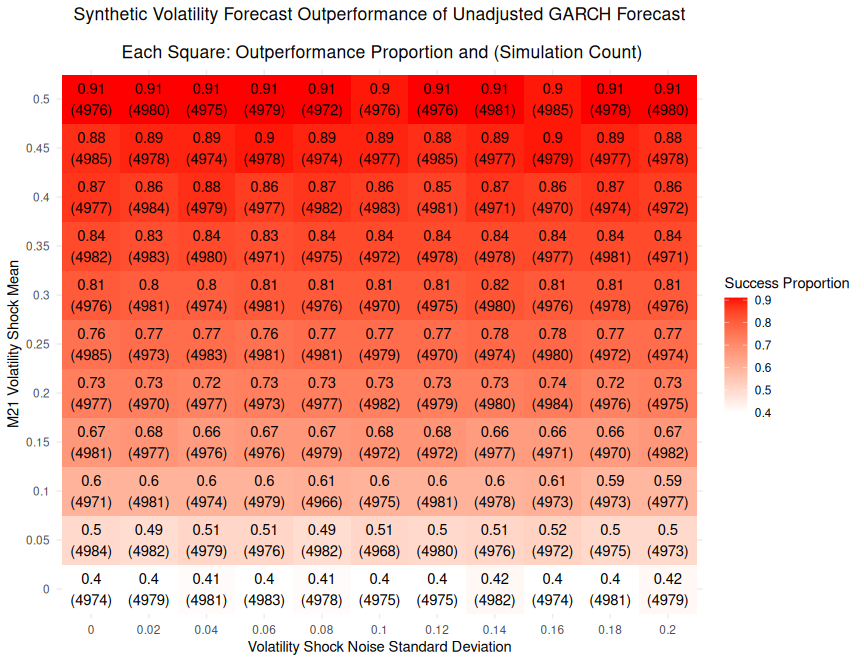
\includegraphics[scale=.45]{simulation_plots/standard_simulation_alpha_.1_beta_.82.png}
    \caption{Fixed parameter values: $\alpha = .1, \beta = .82, \mu_{x} = 1, \sigma_{x} = .1$}\label{fig:heavy_beta}
  \end{center}
  \end{figure}
  
If we switch the values of $\alpha$ and $\beta$, we see similar behavior, as in \ref{fig:heavy_alpha}.  Here we cite \citet[p. 22]{francq2019garch} in motivating simulations for large $\alpha$ values and then large $\beta$ values.  However, for small values of the shock mean, increasing noise does lead to fewer converged simulations, likely due to large negative realizations of the noise term, which in turn lead to near-zero and even negative estimates of the terms $\omega_{i}^{*}$.
\begin{figure}[h!]
  \begin{center}
    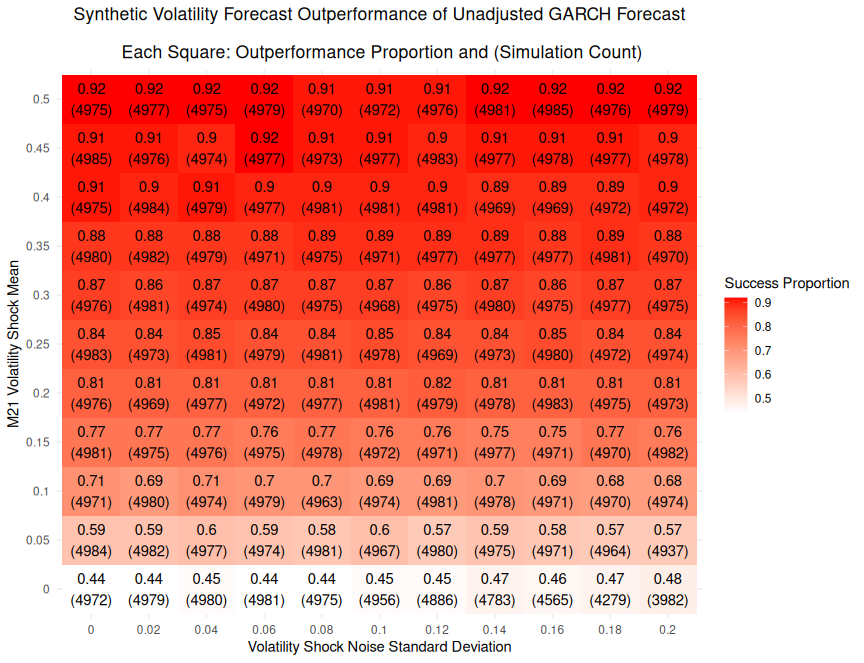
\includegraphics[scale=.45]{simulation_plots/standard_simulation_alpha_.82_beta_.1.png}
    \caption{Fixed parameter values: $\alpha = .82, \beta = .1, \mu_{x} = 1, \sigma_{x} = .1$}
    \label{fig:heavy_alpha}
  \end{center}
  \end{figure}

  % https://tex.stackexchange.com/questions/37581/latex-figures-side-by-side
  \begin{figure}[h!]
    \centering
    \begin{subfigure}{.5\textwidth}
      \centering
      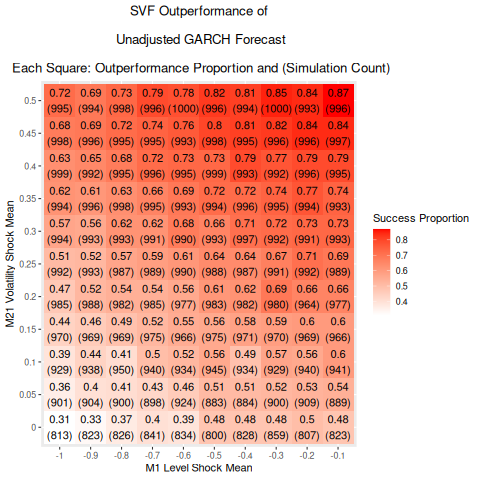
\includegraphics[scale=.45]{simulation_plots/dual_level_vol_shock_FriFeb0911:03:49PM2024.png}
      \caption{$\alpha = .1, \beta = .82, \mu_{x} = 1, \sigma_{x} = .1$}
      \label{fig:dual_shock_strong_betas_inside}
    \end{subfigure}%
    \begin{subfigure}{.5\textwidth}
      \centering
      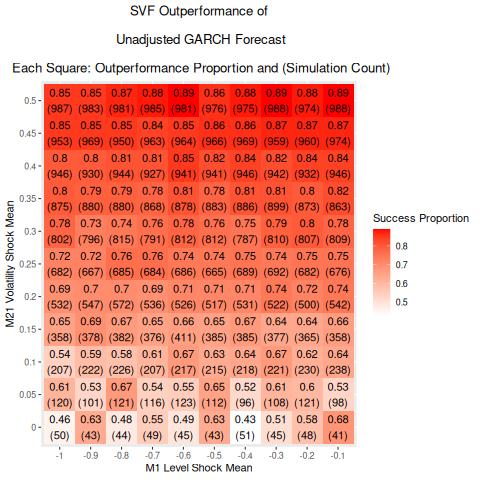
\includegraphics[scale=.45]{simulation_plots/dual_level_vol_shock_FriFeb0911:27:59PM2024.png}
      \caption{$\alpha = .82, \beta = .1, \mu_{x} = 1, \sigma_{x} = .1$}
      \label{fig:dual_shock_strong_alpha_inside}
    \end{subfigure}
    \caption{Shocks to both the mean function and the volatility equation}
    \label{fig:not_sure_what_write}
    \end{figure}

\begin{comment}
  \begin{figure}[h]
  \begin{center}
    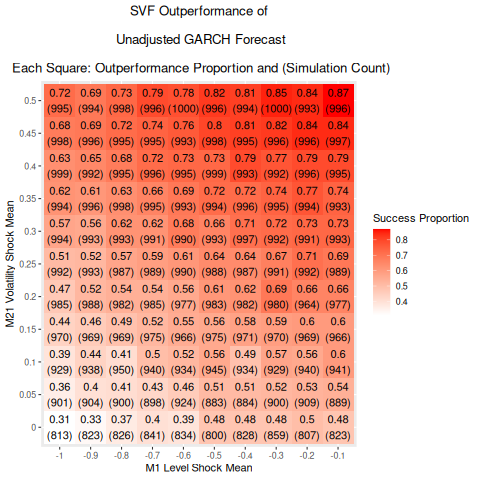
\includegraphics[scale=.75]{simulation_plots/dual_level_vol_shock_FriFeb0911:03:49PM2024.png}
    \caption{Dual shock: both a level and volatility shock at $T^{*}+1$, where fixed parameter values are $\alpha = .1, \beta = .82, \mu_{x} = 1, \sigma_{x} = .1$}
    \label{fig:dual_shock_strong_beta}
    \end{center}
  \end{figure}

\begin{figure}[h]
  \begin{center}
    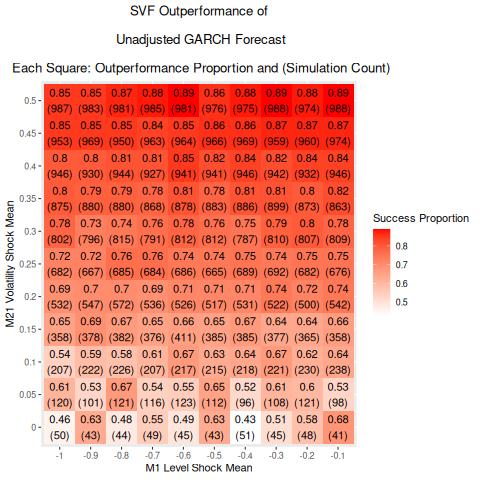
\includegraphics[scale=.75]{simulation_plots/dual_level_vol_shock_FriFeb0911:27:59PM2024.png}
    \caption{Dual shock: both a level and volatility shock at $T^{*}+1$, where fixed parameter values are $\alpha = .82, \beta = .1, \mu_{x} = 1, \sigma_{x} = .1$}
    \label{fig:dual_shock_strong_alpha}
    \end{center}
  \end{figure}
\end{comment}

\begin{comment}
\subsubsection{Length of the Volatility Shock}
\subsubsection{Length of the Level Shock}

\subsubsection{Shorter Series}

\subsubsection{Fat tails in innovations}

\subsubsection{Lengthening the measurement period}

\subsubsection{Changing the optimization norm for distance-based weighting}

\subsubsection{Asymmetric GARCH}
\end{comment}

\clearpage 

\section{Real Data Example}

We show the applicability of our method using a real data example that sits at the crossroads of financial trading and electoral politics.  In the spring of 2016 in the United States, the Republican Party's primary election process narrowed down candidates until Donald J. Trump cleared the threshold of votes to win the nomination formally at the party's convention that summer.  He would go on to face the Democratic Party's nominee, Hillary Rodham Clinton.   

From an ex-ante perspective, several qualities of the 2016 US election cycle as well as the candidates themselves made the election difficult to prognosticate.  The Electoral College permits victory without a majority or even plurality of the popular vote, which can render presidential races more competitive than a raw vote total would, elevating the uncertainty surrounding the country's future leadership.  The election featured no incumbent, ruling out any incumbent-advantage of the empirical, ``statistical" kind distinguished by \citet{mayhew2008incumbency}.  The Republican Party candidate espoused unorthodox, populist positions on matters such as healthcare, trade, and foreign policy, some of which could be considered rare in either of the major two parties.  Additionally, Donald J. Trump, lacking any experience in government --- either electoral or appointed service --- possessed neither a voting record nor any on-the-job performance for voters to judge or his opponents to attack. As one financial industry professional commented, comparing the 2016 election to the upcoming 2024 election, ``this time the markets will be aware of both possibilities and price them to some extent — we wouldn’t expect the same volatility as we saw in 2016 after the election" \citep{News_2024}. Gleaning signals from financial options markets and betting markets, \citet{wolfers2016financial} predicted that markets would decline prodigiously following a Trump victory in November 2016.  Finally, the election outcome delivered significant ``news", in the econometric sense of the word, in the simple sense that it was not predicted.  \citet{goodell2013us} found support for the theory that the polling-implied probabilities of election outcomes encode information about future macroeconomic conditions, which is itself reflected in market volatility.  In its final post before the election result, acclaimed forecasting outfit 538, headed by economist Nate Silver, predicted a Clinton victory with a probability of .714, more than 2-to-1 odds \citep{Silver_2016}, suggesting that Trump's victory was at least somewhat surprising.  

For all of these reasons and more, the aftermath of the 2016 presidential election meets the standard of an interesting and notable event for which a quantitative researcher might seek a volatility point prediction.  On a more technical level, the election outcome was not known until the evening of election day, well after the closing of financial markets at 4pm Eastern Time.  This satisfies the condition that the shock be not yet digested by liquid markets.  We therefore proceed to make the following technical specifications in order to predict the volatility of financial services ETF IYG\footnote{It has been noted that GARCH effects are more attenuated in aggregated returns \citep{zivot2009practical}, which suggests against using the S\&P 500 or similar indices as an example.} (an ETF composed of American financial majors JPMorgan, Bank of American, etcetera) on Wednesday November 9th, 2016.

\begin{enumerate}
    \item \textbf{Model choice} We assume a GARCH(1,1) for the daily log return series of IYG in each donor.  As argued in \citet{hansen2005forecast}, a GARCH(1,1) is rarely dominated by more heavily-parameterized GARCH specifications.  It thus provides a defensible choice when motivation or time for choosing another model is lacking.  For the time series under study and the donor series alike, we fit a GARCH(1,1) on almost four years of market data prior to the shock.

    \item \textbf{Covariate Choice} We choose covariates that could plausibly satisfy the model assumptions spelled out earlier, that is, risk-related and macroeconomic covariates that could plausibly be weighted and summed in a shock distribution.  We thus choose the log return Crude Oil (CL.F), the VIX (VIX) and the log return of the VIX, the log returns of the 3-month, 5-year, 10-year, and 30-year US Treasuries, as well as the log return of the most recently available monthly spread between AAA and BAA corporate debt, widely considered a proxy for lending risk \citep{goodell2013us, kane1996p}.  We also include the log return in the trading volume of the ETF IYG itself, which serves as a proxy for panic.  Finally, we include the squares of the demeaned log return of IYG for the 30 trading days preceding the shocks.  For each variable in the volatility profile, we compute the sample mean and sample standard deviation across the $n+1$ events, allowing us to scale the variables to have zero mean and unit variance.  Hence, no single variable should dominate the distance-based weighting procedure.

    \item \textbf{Donor pool construction} Synthetic Control, as a tool of causal inference, often goes about weighting control units by first identifying a natural set of donors or standard donors such as the untreated units within a set of subnational units like US states or Spanish provinces \citep{abadie2003economic, abadie2010synthetic}.  While such a procedure does not necessarily preclude considered judgments (e.g. should Canadian provinces be used as donors for a treated US state?), as a tool of small-$n$ prediction, distanced-based weighting may favor somewhat different considerations in constructing a donor pool. 
    
    For our purposes, we choose the three most recent US presidential elections prior to the 2016 election.  The three US presidential elections are the only presidential elections since the advent of the ETF IYG.  We exclude the midterm congressional elections in the US (i.e. those held in even years not divisible by four), which generate far lower voter turnout and feature no national races.

    \item \textbf{Choice of estimator for volatility} We use the sum of squared 5-minute log returns of IYG on November 9th, 2016, otherwise known as the Realized Volatility estimator of volatility \citep{andersen2008realized}, as our proxy.  We exclude the first five minutes of the trading day, resulting in a sum of 77 squared five-minute returns generated between 9:35am and 4pm.
\end{enumerate} 

\begin{figure}[H]
\begin{center}
  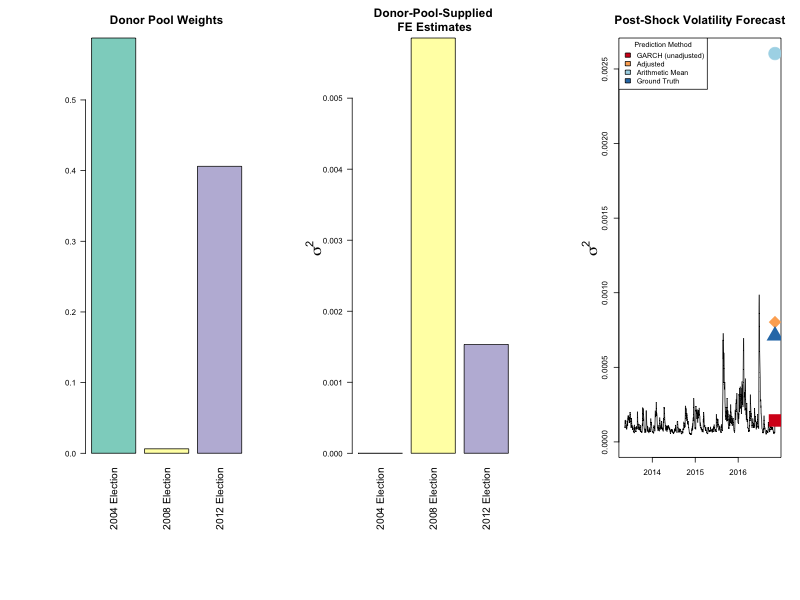
\includegraphics[scale=.5]{real_data_output_plots/savetime_SatMay112045002024_IYG_CL=F-^VIX-^IRX-^FVX-^TNX-^TYX_^VIX_2016-11-08-2004-11-02-2008-11-04-2012-11-06.png}
  \caption{The volatility induced by the 2016 US election}
  \label{fig:SVF_2016}
  \end{center}
\end{figure}

We now discuss the three subplots in Figure \ref{fig:SVF_2016} in order from left to right.  On the left, we see that distanced-based weighting places nearly equal weight on the 2004 and 2012 elections, with only neglible weight on the 2008 election, when financial market conditions were extreme across nearly every dimension.  Assuming an approximately correct specification of the covariates, this is interpreted to mean that even of the 2016 US election had a general climate of risk and tension less extreme than 2008 and more similar to the 2004 and 2012 elections.  In the middle plot, we notice that the fixed effect estimates for 2008 and 2012 are considerable, with only 2004 registering a near-zero fixed effect estimate.  The fixed effect estimates quantify the amount of surprise the US election results delivered (strictly speaking, not only the presidential race but all November elections in the US with the ability to influence financial markets) under the assumption of a GARCH(1,1).  As estimates gleaned from only one data point per time series, they are theoretically high in variance.  On the right, we observe in black the  $\hat\sigma^{2}$ yielded by the GARCH(1,1) for the time series under study.  We also observe four points, all indicated by the legend: three predictions and the ground truth.  We include the prediction derived by adjusting the GARCH(1,1) prediction by the arithmetic mean of the fixed effect estimates.  As is evident, our method comes reasonably close the ground truth.  The prediction is not only directionally correct, i.e. we predict a volatility spike where there is one; the prediction far outperforms the unadjusted prediction.  Remarkably, the arithmetic-mean based prediction here demonstrates the inherent risk in failing to weight each donor appropriately.  The 2008 election receives far more weight than is called for, as simple averaging ignores the radically different conditons on the evening of those two events.  

Naturally, one might ask how sensitive this prediction is to at least two kinds of model specification: donor pool specification and covariate specification.  There are two responses to these concerns.  First, although the practitioner lacks a priori knowledge of the adequacy of the donors with respect to the time series under study, it is possible to gauge the diversity of the donor information by examining the singular values of the volatility profile.  In the prediction presented here, no singular value represents more than 50$\%$ of the sum of singular values.  Indeed, the first four singular values descend from 62$\%$ to 23$\%$ to 15$\%$ of the the cumulative variation, indicating a moderate concentration or redundancy of information in the three donors.  Second, we follow \citet{steegen2016increasing} in a executing a multiverse analysis.  In particular, in the supplement, we carry out leave-one-out analyses on both the donor set and the covariate set.  Additionally, in the supplement, we show that with Brexit added as a donor, the results are unchanged, due to the fact that Brexit's covariates do not lie in the convex hull of the 2004 Election, the 2012 Election, and the time series under study.

\begin{figure}[H]
\begin{center}
  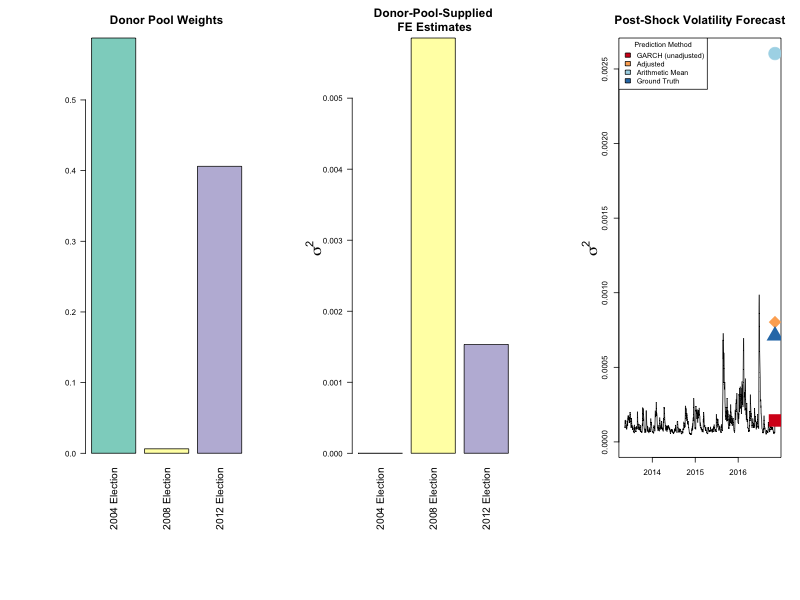
\includegraphics[scale=.6]{real_data_output_plots/savetime_SatMay112045002024_IYG_CL=F-^VIX-^IRX-^FVX-^TNX-^TYX_^VIX_2016-11-08-2004-11-02-2008-11-04-2012-11-06}
  \label{fig:SVF_2016_without_Brexit}
  \end{center}
\end{figure}


\section{Discussion}

This present work extends \citet{lin2021minimizing} principally by substituting the GARCH model for an AR(1), i.e. modeling both the mean and volatility of a univariate time series.  We permit both shocks in the mean model and volatility model of GARCH.  As ancillary improvements, the current work permits the shock periods to be of any length, formally $L_{\text{vol}}, L_{\text{return}} \in\{0,1,2,...\}$, and the weights applied to the donor pool can come from more exotic subsets of $\mathbb{R}^{n}$.  At a more technical level, the most substantial insight related to \citet{lin2021minimizing} is that the GARCH model provides an elegant forecast function for squared observations of the time series under study. However, this use-case becomes less attractive in situations where the sign of the time series under study following the shock is uncertain.

The method under development does not strictly require knowledge of the length of the shocks in the donor pool, but correctly sizing up those shock lengths is helpful to proper estimation of the shocks in the donor pool.  An important question remains: even if the donor pool shock lengths are assumed to be known, how do we advise the operator to forecast the time series under study?  For how long is the forecast reliable?  Should we take a convex combination of the donor pool shock lengths?  Or mean? Or minimum of the donor pool shock lengths?
unlike KNN in that are not trying to learn a function, first and foremost.  We are trying to estimate a parameter.

KNN runs into the problem: the curse of dimensionality.  In contrast, large $p$ is not a problem in synthetic methods, because the thing estimated is the vector $w$ with $n-1$ degrees of freedom.  For KNN, a high-dimensional space, i.e. large $p$, corresponding to many covariates, is a difficult space in which to work with distances \citep{hastie2009elements}.  In contrast, large $p$ is not a problem in and of itself for synthetic control --- in fact, asymptotic results exist for $p$ \citep{abadie2010synthetic}.  

As is pointed out in \citet{hastie2009elements}, KNN regression performs well when $K$ is chosen small enough that one can simply average the points $\{y_{i}\}_{i=1}^{N_{train}}$in the neighborhood around each $\{y_{i}\}_{i=1}^{N_{test}}$ to get good predictions.  As we have noted above, the arithmetic mean-based estimator of $\omega^{*}$, denoted $\overline{\omega^{*}}$, corresponds to KNN when $K = n$, the number of donors.  Fundamentally, the idea that $n$ is small enough and the donors are homogeneous enough that one could simply average the $\hat\omega_{i}$ is at odds with the assumed variation in the shock effects.

In KNN regression, the hyperparameter K must be learned.  In similarity-based parameter correction, the number of donors is not learned.  A donor pool is curated, and then careful rules of thumb can be applied to determine whether a given donor should be included or excluded.  While it would not necessarily hurt to `learn' the appropriate number of donors to use, this information would probably not be as useful as knowing which donors and covariates provide the basis for the best forecasts.  This brings us to a deeper point about the distinction between similarity-based methods in the style of \citet{lin2021minimizing} and KNN.  In KNN, the exogenous variables are taken as a given and `nearness' to object-to-predict depends on the distance function chosen.  In contrast, in \citet{lin2021minimizing}, the determination of nearness begins with a qualitative step, i.e. curating the units between which we will calculate distances and from we will ultimately derive weights.

Should we gather as many donors as possible and pick them quantitatively?  It would be counter to the method proposed to assemble a vast number of donors, lacking careful scrutiny of the qualitative fit, and let the optimization simply pick the donors, via weighting.  What makes a donor good is not merely its quantitative fit but its qualitative fit as well.

\citet{abadie2022synthetic} make a similar point about large donor pools.  What matters is that the donors chosen are properly situated in the $p$-dimensional predictor space, so as to allow proper estimation of the weights.

\begin{comment}
  
\subsection{If we assume knowledge of the covariates that parameterize the shock, why not estimate each parameter individually?}
\textcolor{red}{consider removing}\textcolor{green}{I am considering moving this to the part where I discuss that the GARCH model is nested inside the factor model from \citet{abadie2010synthetic}.}
\begin{enumerate}
  \item Degrees of freedom is first consideration
  \item Each estimate will be quite noisy.
\end{enumerate}


\subsection{Connection to Stochastic Volatility}
SV stipulates that at any time point, both the return distribution and volatility could each be subject to separate shocks \citep{andersen2010stochastic}. \textcolor{red}{This seems incomplete.}

\end{comment}

\begin{comment}
  This needs to be commented out because the current draft has no way to accommodate concurrent information.
  \item \citet{lin2021minimizing} requires exogenous information to arrive strictly between $T^{*}$ and $T^{*}+1$.  However, we may want to relax this requirement so as to permit the exogenous information to be concurrent with the trading session or end of session on $T^{*}+1$.
  \end{comment}

\subsection{News shock literature review}

We adapt the news shock framework of \citet{kilian2017structural}: \\

$z_{T^{*}+1}^{\text{nonscheduled news shock}} \coloneqq z_{T^{*}+1}^{\text{nonscheduled news}} - \E_{T^{*}}[z_{T^{*}+1}^{\text{nonscheduled news}}]$ \\

In our adapted schema, irregular news shocks are $\mathcal{F}_{T^{*}}$-zero-expectation events governed by a GARCH-X process.  As such, $z_{T^{*}+1}^{\text{irregular news shock}}$ admits of the decomposition $z_{T^{*}+1} = \sigma_{T^{*}+1}\epsilon_{T^{*}+1}$. \textcolor{red}{This seems incomplete.}


\begin{comment}
\section{Connection to Signal Recovery}

\begin{table}[]
\begin{tabular}{|p{1.2in}|p{1.9in}|p{1.9in}|}
\hline
  & $\Sigma_{\delta} = I_{p}$ & $\Sigma_{\delta} \neq I_{p}$  \\ \hline
 $\Sigma_{x_{i,T^{*}}} = I_{p}$ & Easiest to model & Captures reasonable possibility of non-zero correlation in random effects \\ \hline
 $\Sigma_{x_{i,T^{*}}} \neq I_{p}$ & Captures empirically-verified phenomenon of non-zero correlation in covariates & Implausibly complicated to model  \\ \hline
\end{tabular}
\end{table}

\begin{table}[h!]
\begin{tabular}{|p{1.3in}|p{1.6in}|p{1.9in}|p{1.9in}|}
\hline
 & Vershynin (2018) & Lin and Eck (2021) & SynthVolForecasting \\ \hline
observed quantity& $y_{i}$  & NA & NA \\ \hline
estimated quantity&  NA& $\alpha_{i}$ &  $\omega^{*}_{i}$\\ \hline
signal & $A_{i}x$ & $\mu + \delta'x_{i,T^{*}}$ & $\mu + \delta'x_{i,T^{*}}$  \\ \hline
prior information & $x\in T$, $T$ a convex & across donors, linear shock function equal in distribution  &  across donors, linear shock function equal in distribution \\ \hline
key assumption(s) & $A_{i}$ independent $\forall i$, isotropic too? & $x_{i,T^{*}}$ independent across donors; independent entries of $x_{i,T^{*}}$ & $x_{i,T^{*}}$ independent across donors; independent entries of $x_{i,T^{*}}$ \\ \hline
noise& w & $\t\varepsilon$  & $\t\varepsilon$   \\ \hline
strategy& Observe $y_{i}$; then estimate $x$ with small expected L2 loss & Estimate $\alpha_{i}$ for $i = 2,...,n+1$; then take convex combination to predict $\alpha_{1}$  & Estimate $\omega^{*}_{i}$ for $i = 2,...,n+1$; then take convex combination to predict $\omega^{*}_{1}$ \\ \hline
\end{tabular}
\end{table}

\end{comment}



\begin{comment}
  
\subsection{News Sentiment}
Within the vast literature on financial sentimental analysis, there exists a sub-literature on financial volatility forecasting using news and news sentiment \citep{atkins2018financial}.  The setting herein is one where the valence of the sentiment is reasonably well-understood, and hence the direction of volatility can be well-predicted, although not perfectly, by human intuition.
\end{comment}

\section{Supplement}

\subsection{Sensitivity to Covariates Chosen}
As mentioned in \ref{}

\subsection{Sensitivity to Donors Chosen}

\subsubsection{Brexit}
We analyze the real-data example with Brexit included and using the daily return in the Pound-Dollar exchange rate as a covariate. \\

Note that by inspecting the fit of the distance-based weighting approximation quantitatively, we can gain some degree of foresight into how well the forecast will be.

\begin{figure}[H]
  \begin{center}
    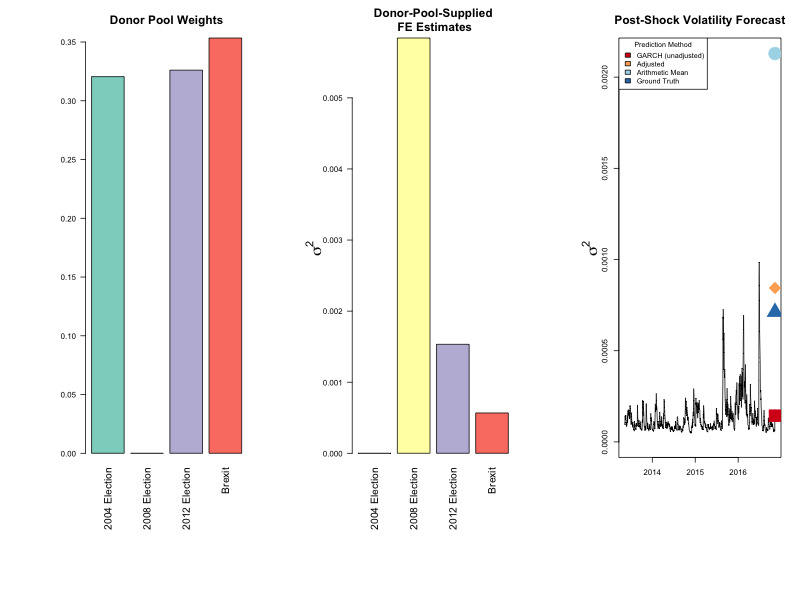
\includegraphics[scale=.6]{real_data_output_plots/savetime_SatMay112046072024_IYG_CL=F-^VIX-^IRX-^FVX-^TNX-^TYX_^VIX_2016-11-08-2004-11-02-2008-11-04-2012-11-06-2016-06-22.png}
    \label{fig:SVF_2016_with_Brexit}
    \end{center}
  \end{figure}

\clearpage

\bibliography{synthVolForecast}

\end{document}